\documentclass{comjnl}

\usepackage{amsmath}

\begin{document}


\title[Modelling Bidders in Sequential Automated Auctions]{3D Keypoint detection with Deep Neural Networks}
\author{El\'{i}as J. Puma}
\affiliation{Escuela Profesional de Ciencia de la Computaci\'{o}n,\\
Universidad Nacional de San Agust\'{i}n,\\
Arequipa, PE}
\email{eliasj.puma@gmail.com}

\shortauthors{E. Puma}

%\received{00 January 2009}
%\revised{00 Month 2009}


%\category{C.2}{Computer Communication Networks}{Computer Networks}
%\category{C.4}{Performance of Systems}{Analytical Models}
%\category{G.3}{Stochastic Processes}{Queueing Systems}
%\terms{Internet Technologies, E-Commerce}
\keywords{Keypoint detection; Deep Neural Networks; 3D Model; Sparse Autoencoders}


\begin{abstract}
3D keypoint detection plays a fundamental role in the Computer Vision field, detection of these salient points in the local surfaces of a 3D object is important in order to perform certain tasks such as registration, retrieval and simplification. There has been a lot of research in the field of 3D keypoint detection, most of them take a geometrical approach which have a good performance but lack flexibility to adapt to changes such as noise and high curvature points that are not keypoints to human preference. A good approach seems to be machine learning methods that can be trained with human annotated training data. In this paper a new method is proposed using deep neural network with sparse autoencoder as the regression model due to their great ability for feature processing. The analysis shows this method would outperform other methods that are widely used.  
\end{abstract}

\maketitle


\section{Introduction}
Several computer-dependent areas are benefited of the applications
that 3D Models have in them. The growth of 3D data has increased in
the last years with the availability of low-cost 3D capture devices~\cite{harris3D}.
The ability to analyse, proccess and select relevant information
from them is an active research area. 

3D interest point detection is a difficult task for several reasons~\cite{Discrim, harris3D}. 
First, there are not any definitions for what a interest point is, 
most of the approaches consider the high level of protusion in a local
area as a keypoint characteristic. So, in planar sections of an area
vertices have a low interest level and in local areas with diferent
structures the interest level will be the opposite. Second, vertex 
density is different for every 3D model which makes harder the task of
selecting a local area. Third, information obtained from a 3D model
are only vertex positions and connectivity between them which means
the interest level will depend only from the information we can
retrieve from different calculations. These are not the only reasons
but are sufficient for explaining why this method is prepared to
handle these difficulties. 

The common approach to 3D keypoint detection has been to use 
geometric properties of the models, although in recent years researchers
also have developed machine learning techniques that try to outperform the
former one by avoiding the problems of: Different tasks in different areas
of the model~\cite{DNN}, false positives obtained from noise or local
variation and keypoint detection valuable according to human preference. 

The rest of this paper is organized in the following way:
Section~\ref{RelatedWork} introduces previous work done in the area,
Section~\ref{Proposal} presents the idea this method is based on. Future
results will be presented in Section~\ref{Results} and future conclusions
in Section~\ref{Conclusions}.

\section{Related Work} \label{RelatedWork}
In recent years researchers have proposed several techniques for
3D keypoint detection. Most of them are based on geometric methods, for
example Sipiran and Bustos extended the Harris operator for 3D
meshes~\cite{harris3D}. Lin, Zhu, Zhang and Liu proposed a geometric
technique~\cite{GMSR} based in the tangencial planes traced for each vertex and
other transformations in the mesh some of them can be also found
in~\cite{DNN}. 

\section{Proposal} \label{Proposal}
This work is inspired by the work of~\cite{DNN} by the use of
sparse autoencoders as the regression model in order to learn features
from local and global information generated from a human-annotated
keypoint database. Also this proposal is influenced by~\cite{UnsLearning},
so for us to achieve the 3D keypoint detection we train a 3-layered locally
connected sparse autoencoder similarly to their technique, such
technique's results revealed to be a inexpensive way to develop
high-level features from unlabeled data, from that study this work
presents an adapted architecture for 3D meshes. Taking a different approach
than the other techniques mentioned above, resized and simplified segments
of the 3D mesh will be used as the input for our Deep Neural Network,
this will enable our DNN to learn when one of these segments has inside
a keypoint.

\subsection{Architecture}
This technique can be seen as a set of sparse deep autoencoders that
similarly to~\cite{UnsLearning} has two fields in it: local receptive fields,
pooling normalization (the architecture taken as a base can be seen
on the Figure~\ref{fig:architecture}). Local receptive fields scale the
autoencoder to big inputs, connecting the autoencoder's features to a small
region of the next lower layer. These sublayers are know as filtering and
pooling.

Originally the neurons in the first sublayer were connected to
pixels in all input channels~\cite{UnsLearning}, but in order to adapt
this architecture it is proposed to use the 3D vertices and their
connectivity information as the input channels and by so adding more
receptive fields.

\begin{figure}
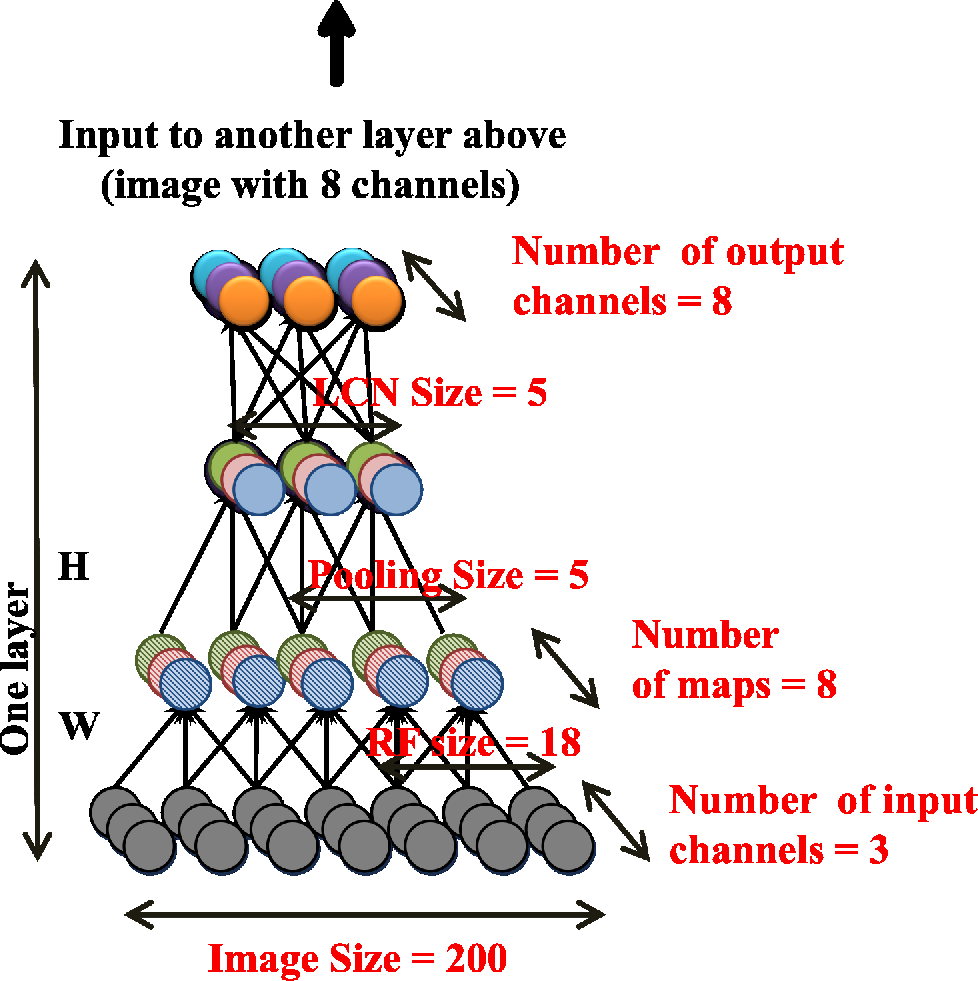
\includegraphics[width=0.9\linewidth]{architecture.png}
\caption{Large scale unsupervised learning architecture \cite{UnsLearning}}
\label{fig:architecture}
\end{figure}

\subsection{Training}
As mentioned before the first layer input...

To train the Deep Neural Network what is to be done at first is to train each
Sparse Autoencoder and a final logistic regression layer, then following the
schema from~\cite{DNN} stack the four layers together and backpropagate the
whole DNN to fine tune it.

The goal of this approach is to reduce the proccessing that is performed,
instead of evaluating each vertex in the DNN which is expensive, we can
perform the neccesary calculations just for some samples of the 3D object
and discard if those samples don't contain any keypoints, in the case we find
the presence of keypoints we will perform further calculations to choose the
sample keypoint.

\section{Results} \label{Results}

\section{Conclusions} \label{Conclusions}

\ack{This research was undertaken as part of ...}


\nocite{*}

\bibliographystyle{compj}
% \bibliography{ModellingBidders}
\documentclass{comjnl}

\usepackage{amsmath}

%\copyrightyear{2009} \vol{00} \issue{0} \DOI{000}

\begin{document}


\title[Modelling Bidders in Sequential Automated Auctions]{Modelling Bidders in Sequential Automated Auctions}
\author{Kumaara Velan}
\affiliation{Intelligent Systems and Networks Group, Department of
Electrical and Electronic Engineering, Imperial College, London
SW7 2BT, UK} \email{kumaara.velan@imperial.ac.uk}

\shortauthors{K. Velan}

\received{00 January 2009}
\revised{00 Month 2009}


%\category{C.2}{Computer Communication Networks}{Computer Networks}
%\category{C.4}{Performance of Systems}{Analytical Models}
%\category{G.3}{Stochastic Processes}{Queueing Systems}
%\terms{Internet Technologies, E-Commerce}
\keywords{Automated Auctions; Analytical Models; Autonomic
Systems; Internet Technologies; E-Commerce; Queueing Systems}


\begin{abstract}
Auctions are mechanisms that formalise the rules with which
automated trading schemes can be conducted, and in this paper we
model the interaction of bidder and seller agents in sequential
computerised auctions. We study the outcome of strategies that a
designated ``special bidder'' (SB) may follow in the presence of a
collection of other bidders in an English auction, under the
assumption that the SB can make bids based on its observation of
the ongoing auction as a collective system. In our model, bidding
and sale events are continuous time random processes with discrete
state-space, where the state-space represents the current value of
the most recent bid. We obtain analytical solutions which allow
the evaluation of measures of interest to the SB such as the
probability of winning, the savings with respect to the maximum
payable price in the event of a win, and the expected waiting time
to win. We examine the effects of the SB's time to bid, and study
how its decisions may be selected so as to optimise the SB's
measures of interest.
\end{abstract}

\maketitle


\section{Introduction}

Computer systems and the Internet have enabled a wide variety of
automated trading schemes which are in use for stocks,
commodities, derivatives and other financial instruments. More
recently, the Internet has also allowed individuals to buy and
sell various items in an open and easily accessible manner. Thus
we can envisage a future when large parts of the economy will be
driven by sequences of automated and interconnected trading
patterns.

Auctions are a convenient mechanism for formalising the rules with
which such automating trading schemes can be conducted, and they
have been widely used for many centuries in human based trading
and commerce. In recent work the stochastic behaviour of
collections of bidders acting in an auction has been analysed
through the use of discrete state-space and continuous time
probability models~\cite{gelenbe06}. The approach constructs
stochastic dynamical models of auctions and bidders, and then
obtains the steady-state behaviour to compute significant
properties of both the ``one-shot'' outcome, and the long-run
repetitive outcome of auctions. One-shot properties include the
probability distribution and the expected sale price, while
long-term properties include the income per unit time obtained by
the seller over a large number of transactions.
In~\cite{gelenbe_inPress} the model has been extended to study a
network of interconnected auctions, where bidders are allowed to
move freely between auctions, and an analytical solution has been
obtained. These mathematical techniques, and their variants, have
also been successfully deployed in other diverse range of problem
areas: from biological applications in modelling populations of
viruses and agents~\cite{Gelenbe-SoftwareViruses}, to
communication systems in minimising packet travel time across a
wireless network~\cite{Gelenbe07_DiffModelPacketTravel,
Gelenbe_06_Workshop_TravelDelay}, and choosing adaptive routing
decisions~\cite{Gelenbe03_Sensible}.

In reality, knowledge of the existence of opportunity and
availability to purchase similar goods in the future may influence
a bidder to choose to forgo the opportunity of procuring a good at
a high cost, and instead wait in the hope of securing a better
deal later. We can also imagine situations where goods are
reusable resources that are not sold per se, but rented out and
returned to the seller at the end of some period, so that bidder
agents who are not in urgent need to obtain a good immediately may
defer a purchase. Interesting work along these lines, where
bidders exhibit rational forward-looking behaviour when deciding
strategies for the current auction can be found in
\cite{zeithammer06}. A possible application for auctions of
reusable goods in allocating computing resources is given
in~\cite{gagliano_etal_95}.

When we discuss automated auctions, we will invariably imagine
software agents representing human counterparts in the digital
marketplace~\cite{maes99}, acting autonomously and yet guided by
its design objectives to fulfill the interests of their owners to
the best possible extent. In such instances it is crucial that the
underlying communications infrastructure is designed to allow and
support the user, i.e. the agent, to set the criteria for its
service requirements. For example, a bidder agent may have certain
specific needs with respect to its connectivity to the seller, and
so may request for a network path with the minimum overall delay
to the seller be established, or an agent physically located on a
mobile node may prefer a connection that consumes the minimum
power, or any weighted combination of its other goals. In this
regard, auctions, or any digital marketplace activity for that
matter, will benefit from autonomic
communications~\cite{Dobson_etal_06} where emphasis is placed to
insulate the user experience and services from changes, whether
predicted or not, to the underlying infrastructure. In particular,
a self-aware network, as proposed and implemented in the
\emph{cognitive packet network}~(CPN)~\cite{Gelenbe_etal_Nagoya,
Gelenbe_Gellman_Su_ISCC03, Gelenbe-Gellman-Lent-Liu04},
accomplishes this by online internal probing and measurement
mechanisms that are used for self-management, so that it adapts
itself to provide the user the best effort quality of service
(QoS). The CPN performs these corrective actions by using random
neural networks with reinforcement
learning~\cite{Gelenbe_01_CompNetw_CPN, Gelenbe_Mascots02,
Gelenbe_Lent_Nunez_04}, and finds newer routes with improved QoS
using genetic algorithms~\cite{Gelenbe_Liu06_workshop,
Gelenbe_Liu06_GeneticAlgorithmsRouteDiscovery}. In a wireless
mobile ad hoc network environment, where power efficiency is an
overriding concern, the CPN has been extended to incorporate
power-awareness~\cite{Gelenbe-Lent_2004}, and the problem of
controlling the admission of new users into the network while
preserving the QoS of all users has been addressed in
\cite{gelenbe_sakellari_08}.

Beyond ensuring QoS for users, at a different level of
abstraction, the ongoing research in autonomic communications has
a broader objective of providing an intelligent platform for
efficient interaction between digital objects such as users and
services~\cite{Gelenbe05_UsersServicesIntNetworks}, or as in our
context between buyer and seller agents. An important aspect of
applying the ``intelligence'', as discussed in
\cite{ferdinando_etal08}, is in creating new knowledge based on
collected raw sensitive data, through a knowledge network which,
in turn, can be used to enhance economic efficiency. In this
example, it is shown that a good allocation efficiency can be
achieved in a trading application where the aggregated knowledge
is used to create new markets so that sellers can respond to
buyers' needs as they arise.


Security is another vital feature in a communication network,
especially when transactions involving e-commerce activities such
as auctions are conducted; the servers running these applications
are easy targets for attackers, either as a malicious act of
sabotage or for profitable gains. The denial of service (DoS)
attack is a particularly critical threat, since it is easy to
launch, and by its usually distributed nature, difficult to
protect against. Thus an autonomic approach to defending the
network, based on self-monitoring and adaptive measures, has been
suggested in \cite{Gelenbe_Loukas07_SelfAwareDoS}, and several
biologically inspired DoS detectors have been evaluated in
\cite{Loukas_Oke_07, Loukas_Oke_LikelihoodRatios,Oke_etal07}.


In this paper we extend the work in~\cite{gelenbe06} to study the
outcome of strategies that a designated bidder may follow in an
English auction, in the presence of a collection of other bidders,
under the assumption that this ``special bidder'' (SB) observes
the parameters resulting from the auction as a collective (many
bidders and the seller) system. Note that in~\cite{gelenbe06}
bidders are lumped together in a pool, where everyone shares a
similar behaviour; whereas in this work we propose a
generalisation in that the SB is allowed to have its own activity
(bidding) rate which may differ from the other bidders', and
examine how the SB should select its bidding rate in a
self-serving manner.

We first sketch the model to be studied, and then in Section
\ref{Model} we analyse it in detail. The manner in which the model
provides performance measures of interest to the SB and to the
seller, is discussed in Section \ref{Performance} where we first
discuss how the SB can behave in order to optimise outcomes that
are in its best interest, and provide  numerical examples to
illustrate the approach and the model predictions. We then explore
how the SB can try to achieve balance and compete with the other
bidders in Section \ref{KeepUp}. Finally Section
\ref{Price-Dependent} generalises the analysis to the case where
the bidding rates depend on the current price attained in the
auction. Conclusions are drawn in Section \ref{Conclusions} where
we also suggest further work.



\subsection{An English auction with $n+1$ competing bidders}\label{Sec:FirstModel}

Consider an English auction in which the SB participates with $n$
other bidders. We assume that a single good is being sold, and
that it has a maximum valuation $v>0$, so that none of the bidders
will bid beyond the sum $v$. Initially we assume that $v$ is a
fixed and identical valuation for all of the bidders, but it is
easy (see \cite{gelenbe06}) to generalise the results to the case
where $v$ is a  random variable so that the actual valuation that
buyers associate with a good is known in terms of the probability
distribution of a random valuation $V$.

During the auction, each bidder may take some time to consider the
current highest offer before deciding to place a new
counter-offer. We assume that these thinking times are
exponentially distributed random variables with parameters $\beta$
and $\lambda$, for the SB and the other bidders, respectively, so
that we may distinguish the behaviour of the SB from all the other
bidders which have a common statistical behaviour. All the bidders
can participate in submitting bids, except obviously for the
bidder who owns the current highest offer. Furthermore we assume
that all bids proceed with unit increments with respect to the
previous bid, in order to minimally surpass previous highest bid.

It should be noted that, by allowing the SB to have its own
bidding rate, our model generalises the previous~\cite{gelenbe06},
and enables us to characterise the system outcomes as a function
of the ``divergence'' of the SB's behaviour from the other
bidders. We examine these outcomes from both the seller's and the
bidder's interests. As we would expect, if there is no divergence,
i.e. we fix $\beta=\lambda$, then this model reduces to the
previous.

Once a bid is received, the seller considers the offer for some
time before accepting. If a higher bid is submitted before this
time expires, then the earlier offer is rejected (and the previous
highest bidder rejoins the bidder pool), while the seller waits
for another random time, represented by an exponentially
distributed random variable with rate parameter $\delta$.

On the other hand, if no new bid arrives by the end of the
seller's waiting time, the auction concludes with a sale to the
current and hence highest bidder, and as in~\cite{krishna02}, the
seller is indifferent to the identity of the bidder.

After the sale is successfully concluded, the seller ``rests'' for
some random time and then the auction repeats itself as a
statistically independent replica with a population of $n+1$
bidders. The rest time can be thought of as the time spent in
declaring the winner, eliciting payment and allocating the item,
followed by the time spent in preparing the next item for sale. We
assume the rest times are exponentially distributed with expected
value $r^{-1}$, and that successive rest times are independent of
all past events. Note that all of our results will hold if we
assume that the rest times obey some general (i.e. not necessarily
exponential) distribution function.

\section{The mathematical model} \label{Model}

The system that we have described is modelled as a continuous time
Markov chain $\{X_t : t \geq 0\}$ with state-space
\begin{equation}\label{eq:statespaceY}
X_t\in Y =\{0, O(l),R(l),A(O,l),A(R,l):1\leq l \leq v\}.
\end{equation}
Initially we have $X_0=0$ and the state valuations are described
as follows for $t\geq 0$:
\begin{itemize}
\item $X_{t}=0$, if no bid is placed at time $t$. Note that this
may occur after any one of the instants
$t_{i+1}=\inf\{t:t>t_i~\textrm{and}~X_{t_{i+1}}=0\}$ when the
seller accepts a bid, and the auction restarts. We set $t_0=0$.

\item $X_{t}=O(l)$ where $0 < l\leq v$, if at time $t$ the current
valuation of the bid is $l$ and the current bidder is not the SB,
regardless of who placed the previous $l-1$ bids.

\item $X_{t}=R(l)$ where $0 < l\leq v$, if at time $t$ the current
bidder is the SB and the valuation of his bid, i.e. the current
highest bid, is $l$.

\item $X_{t}=A(O,l)$, if at time $t$ the auction has concluded
with a sale at price $l$ to one of the ``other'' $n$ bidders, i.e.
other than the SB, and the next auction has not yet restarted.

\item $X_{t}=A(R,l)$, if at time $t$ the auction has concluded
with a sale at price $l$ to the SB, and the next auction has not
yet restarted.

\end{itemize}
Any bidder which is not the current highest bidder can place a bid
at rate $\beta$ and $\lambda$, respectively, for SB and the other
bidders, as long as the current bid valuation has not attained
$v$. When the valuation $v$ has been attained, no further bids
will be placed. Also, the transition rate that denotes the start
of a new auction, from either state $A(O,l)$ or $A(R,l)$ to state
$0$ is $r$, and  the transition rate (denoting the seller's
decision to sell) from state $O(l)$ to $A(O,l)$ and from $R(l)$ to
$A(R,l)$ is $\delta$. Note that the seller cannot tell the
difference between the SB and the other bidders, and the
transition rates in this first model do not depend on the current
valuation of the highest bid.

For any state $x \in Y$, let the stationary probability of the
state be denoted by $P(x) = \lim_{t \to \infty} P \{ ~X_t=x~ \}$;
then the balance equations satisfied by the stationary
probabilities are
\begin{align} \label{eq:1}
&P(O(1)) ((n-1)\lambda + \beta + \delta )=n \lambda P(0), \\
&P(O(l)) ((n-1)\lambda + \beta + \delta)=(n-1) \lambda
P(O(l-1)) \nonumber \\
&\quad\quad+ n\lambda P(R(l-1)) , \quad 2\leq l\leq v-1 ,\nonumber \displaybreak[0]\\
&P(O(v))\delta =(n-1) \lambda P(O(v-1)) + n\lambda P(R(v-1)), \nonumber \displaybreak[0]\\
&P(A(O,l))r=\delta P(O(l)) ,\quad 1\leq l\leq v ,\nonumber \displaybreak[0]\\
&P(R(1)) (n \lambda + \delta)=\beta P(0) , \nonumber \displaybreak[0] \\
&P(R(l)) (n \lambda + \delta)=\beta P(O(l-1)) ,\quad 2\leq l\leq v-1 ,\nonumber \displaybreak[0]\\
&P(R(v)) \delta = \beta P(O(v-1)), \nonumber \\
&P(A(R,l)) r = \delta P(R(l)) ,\quad 1\leq l\leq v ,\nonumber \displaybreak[0] \\
&P(0)(n\lambda+\beta) = r  \sum_{U=O,R}\sum_{l=1}^v P(A(U,l)) , \nonumber \\
&1=P(0)+\sum_{U=O,R}\sum_{l=1}^v \big[P(U(l))+P(A(U,l))\big]
.\nonumber
\end{align}
After some algebra we can write
\begin{align} \label{eq:1_3}
&P(O(l))=H(l) P(0) ,\\
&P(R(l))=G(l) P(0),\nonumber \\
&P(A(O,l))=\frac{\delta}{r} H(l) P(0), \nonumber \\
&P(A(R,l))=\frac{\delta}{r} G(l) P(0),\nonumber
\end{align}
where
\begin{align}
H(l)&=\left\{\begin{array}{l} \displaystyle \frac{n\lambda}{(n-1)\lambda+\beta+\delta} \quad , l=1  \\
\displaystyle \frac{(n-1)\lambda}{(n-1)\lambda+\beta+\delta} H(l-1)  \\
~{+}\:\displaystyle \frac{n\lambda}{(n-1)\lambda+\beta+\delta} G(l-1)~, 2\leq l\leq v-1  \\
\displaystyle \frac{(n-1)\lambda}{\delta}
H(l-1)+\frac{n\lambda}{\delta}
G(l-1)\quad, l=v \end{array} \right. \nonumber \\
G(l)&=\left\{\begin{array}{ll} \displaystyle \frac{\beta}{n\lambda+\delta} &, l=1 \nonumber \\
\displaystyle \frac{\beta}{n\lambda+\delta} H(l-1) \quad & , 2\leq l\leq v-1 \nonumber  \\
\displaystyle \frac{\beta}{\delta} H(l-1) &, l=v
\end{array} \right.
\end{align}
and
\begin{equation}\label{eq:P0_FirstModel}
P(0) = \frac{r\delta}{r\delta+(r+\delta)(n\lambda+\beta)} .
\end{equation}
In the following we will obtain the closed form expression for
$H(l)$ where $1\leq l \leq v-1$. Let us define the constants
\begin{align}
\alpha_1 &= \frac{n\lambda}{(n-1)\lambda+\beta+\delta}, \\
\alpha_2 &= \frac{(n-1)\lambda}{(n-1)\lambda+\beta+\delta},
\nonumber \\
\alpha_3 &= \frac{(n-1)\lambda}{\delta}, \nonumber\\
\alpha_4 &= \frac{n\lambda}{\delta}, \nonumber\\
\alpha_5 &= \frac{\beta}{n\lambda+\delta}, \nonumber\\
\alpha_6 &= \frac{\beta}{\delta}. \nonumber
\end{align}
We can immediately identify the recurrence relation in $H(l)$ by
substituting $G(l)$ with its valuation as a function of $H(l-1)$:
\begin{equation}\label{rec}
H(l) = \alpha_2 H(l-1) + \alpha_1 \alpha_5 H(l-2), \quad 3\leq l
\leq v-1 ,
\end{equation}
with initial values $H(1)=\alpha_1$ and
$H(2)=\alpha_1(\alpha_2+\alpha_5)$. Let $R_1,~R_2$ be the roots of
this recurrence equation, then
\begin{equation}
R_{1,2} = \frac{1}{2} \bigg[~\alpha_2 \pm \sqrt{\alpha_2^2+
4\alpha_1\alpha_5} ~\bigg] \nonumber .
\end{equation}
We then have
\begin{equation}\label{eq:ClosedFormSolution_Hl}
\begin{split}
H(l) &= \frac{1}{2 (R_1-R_2)} \Big[
(-\alpha_2+2\alpha_1+R_1-R_2) R_1^l \\
&\quad + (\alpha_2-2\alpha_1+R_1-R_2) R_2^l \Big]  , \\
&\qquad\qquad\qquad\qquad\qquad 1 \leq l \leq v-1,
\end{split}
\end{equation}
and at the boundary $l=v$, the solution involves a different set
of coefficients:
\begin{equation}
H(v) = \alpha_3 H(v-1) + \alpha_4\alpha_5 H(v-2).
\end{equation}
Since $G(l)$ is defined as a function of $H(l-1)$, we also have
\begin{align}\label{eq:ClosedFormSolution_Gl}
G(1) &= \alpha_5 ,\\
G(l) &= \frac{\alpha_5}{2 (R_1-R_2)} \Big[ (-\alpha_2+2\alpha_1+R_1-R_2 ) R_1^{l-1} \nonumber \\
&\quad + (\alpha_2-2\alpha_1+R_1-R_2) R_2^{l-1} \Big] ,\;  2 \leq
l \leq v-1 ,
\nonumber\\
G(v) &= \alpha_6 H(v-1)  .\nonumber
\end{align}

Notice that because all the $\alpha_i>0$,
$\alpha_2^2+4\alpha_1\alpha_5>0$ and
$R_1-R_2=\sqrt{\alpha_2^2+4\alpha_1\alpha_5}>0$, we are assured of
the solution of these equations. Also, if the valuation $v$ is
replaced by a random variable $V$ with some general distribution
function $Prob[V=v]=p(v)$ both for the SB and the other bidders,
then the analysis follows directly from the previous discussion by
computing expectations with respect to the random variable $V$.

\section{Performance measures of interest to the SB and to the seller}  \label{Performance}

Some measures of interest to the SB are:
\begin{enumerate}
\item \label{Perf1}whether the SB is actually able to purchase the
item it is seeking, \item \label{Perf2} how quickly it can
purchase the item, \item \label{Perf3} whether it is able to
minimise the cost of its purchase or equivalently how much it
saves with respect to the maximum price that it is willing to pay,
and what is its savings per unit time with respect to the maximum
price $v$ that it might have paid.
\end{enumerate}
On the other hand, the seller's interest may be to maximise its
income from a sale, or to maximise its {\em income per unit time}
for a sequence of sales.

Note that $P(0)$ is the ratio of the average time elapsing from
when the auction starts until the first bid arrives, to the total
average time $\tau$ an auction cycle lasts (including the ``rest
time'' of average valuation $r^{-1}$ after an auction ends). Since
the system leaves state $0$ only when the first bid in an auction
is made, the average time spent in this state is simply the
inverse of the rate at which the first bid is made, i.e.
$[n\lambda + \beta]$, and
\begin{align} \label{eq:FirstModel_P0Definition}
P(0)&=\frac{\text{Average time in state } 0}{\tau}  \\
\tau&=\frac{P(0)^{-1}}{n \lambda+\beta}\nonumber \\
&=\frac{r\delta+(r+\delta)(n\lambda+\beta)}{r\delta(n\lambda+\beta)}
\nonumber.
\end{align}
When a sale is made, the {\em expected income of the seller} is
\begin{equation}
I = \frac{ \sum_{l=1}^v l[P(A(R,l))+P(A(O,l))]}{ \sum_{l=1}^v
[P(A(R,l))+P(A(O,l))]} ,
\end{equation}
and {\em the seller's income per unit time} is
\begin{equation}
\iota = \frac{I}{\tau} \,.
\end{equation}

Concerning (\ref{Perf1}),  the {\em probability that the SB is the
bidder that makes the purchase} at an auction, rather than one of
the other bidders, which we denote by $\pi$, it is given by
\begin{align} \label{eq:pi_WinningProb}
\pi &=\frac{\sum_{l=1}^{v} P(A(R,l))}{\sum_{l=1}^{v}[P(A(R,l))+P(A(O,l))]} \\
&=\bigg[\sum_{l=1}^{v} P(A(R,l)) \bigg] \cdot \bigg[
\frac{r}{n\lambda+\beta} [P(0)]^{-1} \bigg] \nonumber \\
&=\bigg[\sum_{l=1}^{v} P(A(R,l))\bigg] \cdot \bigg[
\frac{r\delta+(n\lambda+\beta)(r+\delta)} {\delta(n\lambda+\beta)}
\bigg]. \nonumber
\end{align}
Hence regarding (\ref{Perf2}) {\em the average time $\psi$ that
the SB waits to win} an auction is the inverse of its winning rate
or
\begin{equation} \label{eq:FirstModel_ExpWaitToWin}
\psi(v)=\frac{\tau}{\pi}=\frac{1}{r\sum_{l=1}^{v}P(A(R,l))} \,.
\nonumber
\end{equation}
Concerning (\ref{Perf3}) {\em the average difference between the
valuation $v$ for the good, and the price at which the auction
concludes given that the SB makes the purchase}, is denoted by
\begin{equation} \phi(v)\ = \frac{ \sum_{l=1}^{v} (v-l) P(A(R,l))
}{ \sum_{l=1}^{v}P(A(R,l))} \,.
\end{equation}

\subsection{Optimisation on the part of the SB}

All that the SB can do, without reverting to deceit, is to adjust
its bidding rate $\beta$ to the situation it is observing,
including the bid rate it observes concerning other bidders, so as
to optimise the performance measures that it is selfishly and
legitimately interested in.

In order to minimise $\psi(v)$ it would suffice to take
$\beta>>n\lambda$. Then the SB raises its bid to the valuation $v$
very quickly so that it is always the winner, and $\pi(v)$ tends
to $1$. However this means that the SB would be buying the good at
its maximum price, rather than driving a good bargain.

Thus a reasonable approach would be to choose a valuation of
$\beta$ which maximises the SB's return on the auction, such as
$\gamma(v)$, the average savings per unit time that the SB makes
with respect to the maximum price that it would pay, or
specifically
\begin{equation}
\gamma(v) = \frac{\phi(v)}{\psi(v)} = r \sum_{l=1}^v
(v-l)P(A(R,l)).
\end{equation}
If $v$ is replaced by the random variable $V$, the function of
interest to the SB is
\begin{equation}\label{SB-objective-av}
\Gamma =E[\gamma(V)]= r\sum_{v=1}^\infty\sum_{l=1}^v
(v-l)p(v)P(A(R,l)),
\end{equation}
and with the previous analysis we have
\begin{equation}
\Gamma = \delta\sum_{v=1}^\infty\sum_{l=1}^v (v-l)p(v)G(l)P(0).
\end{equation}
Hence the SB could choose a valuation of $\beta$ that maximises
$\Gamma$.

\subsection{Numerical examples}

We will now provide some numerical examples that illustrate the
predictions of the model. In all the numerical results that are
shown, we provide curves for the case when all bidders including
the SB follow a symmetric bidding strategy, i.e. $\lambda=\beta$,
and for the more interesting case when the SB varies its bidding
rate while the rest have a fixed bidding rate. The topic of mutual
adaptation of all bidders to each other is yet another important
subject which is not discussed in this paper.

\begin{figure}
\centering
%\includegraphics[width=3in]{model2_ExpTime_SymmetricVsAsymmetric.eps}
\caption{SB's expected time to win with $\delta=0.5$, $r=1$,
$n=10$, $V\sim U(80,100)$.}\label{fig:ExpTime}
\end{figure}

\begin{figure}
\centering
%\includegraphics[width=3in]{model2_ExpPayoff_SymmetricVsAsymmetric.eps}
\caption{SB's expected payoff with $\delta=0.5$, $r=1$, $n=10$,
$V\sim U(80,100)$. }\label{fig:ExpPayoff}
\end{figure}



\begin{figure}
\centering
%\includegraphics[width=3in]{model2_ExpPayoffperTime_SymmetricVsAsymmetric.eps}
\caption{SB's expected payoff per unit time with $\delta=0.5$,
$r=1$, $n=10$, $V\sim U(80,100)$. }\label{fig:ExpPayoffPerTime}
\end{figure}



Comparisons of the asymmetrical bidders case where $\lambda$ is
constant, against the case with identical bidders with
$\lambda=\beta$ are also shown in Figures \ref{fig:ExpTime},
\ref{fig:ExpPayoff}, \ref{fig:ExpPayoffPerTime},
\ref{fig:ExpIncomePerTime}. In Figure \ref{fig:ExpTime}, as we
would expect, we see that in the asymmetric case it suffices for
the SB to bid at a sufficiently high rate (the $x-axis$) in order
to reduce its time until it can make a purchase (the $y-axis$).

In Figure \ref{fig:ExpPayoff} we study the quantity $\phi(v)$. It
is interesting to see that for fixed $\delta$ and $\lambda$, even
if the SB increases $\beta$ to very high valuations (and hence
wins the bid), the ``expected payoff'' $\phi(v)$  {\em does not}
tend to zero and only drops slowly with $\beta$. However, if
$\lambda=\beta$ and they increase, then the pay-off will tend to
zero.

On the other hand, when buyers are interested in purchasing
multiple goods from the auction or when they have a long term view
of things, the expected payoff per unit time $\gamma(v)$ can be a
good criterion for decision making. Figure
\ref{fig:ExpPayoffPerTime}, with the $y-axis$ in logarithmic
scale, shows that the expected pay-off per unit time increases
very rapidly with $\beta$, and furthermore this effect is
accentuated, and the pay-off is greater, when the other bidders
are relatively slower, i.e. have smaller valuations of $\lambda$.
Figure \ref{fig:ExpPayoffPerTime} shows that bidding at a high
rate increases the payoff rate for the bidder and that it leads to
diminishing returns of payoff per time beyond some valuation of
$\beta$. In other words, when the SB's actions do not impact the
other bidders' behaviour, it should bid quickly. This is contrary
to what we observe in online auctions such as eBay, in which
``sniping'' is often used regardless of other bidders' strategies.
Bidders wait until the last possible moment before the auction
expires to place their true bids.

Indeed, it has been suggested that sniping is a good strategy
\cite{roth02,ockenfels06,bajari03} if the information on the
closing time of the auction is made public by the seller. But this
strategy has its shortcomings: in balancing the benefits of
submitting the very last bid against the risk of bid being
rejected for arriving after the auction has ended, the bidders can
misjudge. Technical issues such as communication delay can
aggravate the problem, causing the item to sell at a lower price
than what it can fetch. It is desirable that the time spent in
waiting for the auction to close be shortened, thus saving time
for both seller and bidders; this is especially so when the seller
has many items to sell and time is of the essence. Interestingly
enough, a variant of the auction protocol that was until recently
used by Amazon tackles sniping behaviour by automatic deadline
extension: if any bid is submitted within the last 10 minutes of
the scheduled closing time, the deadline is automatically extended
for another 10 minutes. This process continues until 10 minutes
have passed since the last received bid, at which time the auction
concludes. While it may succeed in discouraging sniping
\cite{ockenfels06}, this approach is not always time effective:
the scheduled deadline is the best-case time within which the
seller can hope to make a sale, and in general it is likely that
it will take longer. This may not be suitable if the seller is
pressed for time. Note also that Amazon has stopped running
auctions as indicated in their Changes to the Participation
Agreement of April 14 2008\footnote{See
\emph{http://www.amazon.co.uk/gp/help/customer/display.html
?ie=UTF8\&nodeId=200239030} that we have accessed on 22-04-2008}.


Finally Figure \ref{fig:ExpIncomePerTime} looks at things from the
perspective of the seller; for fixed $\lambda$ we see that the
SB's bid rate $\beta$ affects the seller's income per unit time,
but only in a moderate way. This is to be expected because after
the SB makes a bid, it must pause and the remaining bidders then
have a chance to bid. Since there are many other bidders (in this
example $n=10$) they will have a significant impact on the
outcome, while the SB's effect remains limited.

\begin{figure}
\centering
%\includegraphics[width=3in]{model2_ExpIncomeperTime_SymmetricVsAsymmetric.eps}
\caption{Expected income per unit time for the seller, with
$\delta=0.5$, $r=1$, $n=10$, $V\sim
U(80,100)$.}\label{fig:ExpIncomePerTime}
\end{figure}



\section{When the SB tries to keep up with other bidders} \label{KeepUp}

An interesting question arises if the SB adjusts its bidding rate
$\beta$ in a manner proportional to the bidding rate of all other
bidders. From the state equations (\ref{eq:1}) we can set a value
$\mu$ representing the relative rate at which both SBs and other
bidders are bidding, with respect to the other bidding and
decision rates. Thus the quantity $\mu$ illustrates the
``similar'' behaviour of SBs and of the other bidders, and we have
\begin{equation}
\mu\equiv\frac{\beta}{n\lambda+\delta}=\frac{(n-1)\lambda}{(n-1)\lambda+\beta+\delta}
\,. \nonumber
\end{equation}
Then, the outcome of the auction for the SB will be equivalent to
that for the other bidders taken together. In fact if $n$ is large
enough, this simplifies to
\begin{equation}\label{eq}
0 = \beta^2+\beta[n\lambda+\delta]-n\lambda[n\lambda+\delta],
\end{equation}
which yields
\begin{equation}
\beta\approx\frac{n\lambda+\delta}{2}\bigg[\sqrt{1+4\frac{n\lambda}{n\lambda+\delta}}
-1\bigg], \label{beta}
\end{equation}
or
\begin{equation}
\mu\approx\frac{1}{2}\bigg[\sqrt{1+4\frac{n\lambda}{n\lambda+\delta}}
-1\bigg] .\label{mu}
\end{equation}


Figure \ref{fig:ExpTime_SBKeepUp_VaryLambda} shows our model's
predictions on the expected time to win for SB, while in figures
\ref{fig:ExpPayoffPerTime_SBKeepUp_VaryLambda} and
\ref{fig:ExpIncomePerTime_SBKeepUp_VaryDelta} we show the payoff
and income rates, respectively, as functions of varying $\lambda$
and $\delta$, when SB follows this policy in keeping up with the
other bidders. In Figure \ref{fig:ExpTime_SBKeepUp_VaryLambda},
for each case of $n$, there exists a minimum expected time to win
that occurs at some $\lambda$, and for increasing $n$ this minimal
point occurs at smaller $\lambda$. Likewise, the highest payoff
per time is obtained at a distinct valuation of $\lambda$ and this
decreases with $n$. These observations correspond to increasing
competition with $n$, and the penalty suffered by SB for an
increase in $\lambda$ is larger for systems with large $n$; the
drop in payoff per time is increasingly steeper with $n$ (see
Figure~\ref{fig:ExpPayoffPerTime_SBKeepUp_VaryLambda}). On the
other hand, the seller benefits from large $n$ and its income per
time has higher peaks, as shown in
Figure~\ref{fig:ExpIncomePerTime_SBKeepUp_VaryDelta}.

\begin{figure}
\centering
%\includegraphics[width=3in]{ExpTime_SBKeepUp_VaryLambda.eps}
\caption{Expected time to win for SB when keeping up with the
other bidders for various $\lambda$ and $n$. Other parameters:
$\delta=0.5$, $r=1$.}\label{fig:ExpTime_SBKeepUp_VaryLambda}
\end{figure}


\begin{figure}
\centering
%\includegraphics[width=3in]{ExpPayoffPerTime_SBKeepUp_VaryLambda.eps}
\caption{Expected payoff per time for SB when keeping up with the
other bidders for various $\lambda$ and $n$. Other parameters:
$\delta=0.5$,
$r=1$.}\label{fig:ExpPayoffPerTime_SBKeepUp_VaryLambda}
\end{figure}


\begin{figure}
\centering
%\includegraphics[width=3in]{ExpIncomePerTime_SBKeepUp_VaryDelta.eps}
\caption{Expected income per time for the seller when SB keeps up
with the other bidders for various $\delta$ and $n$. Other
parameters: $\lambda=1$,
$r=1$.}\label{fig:ExpIncomePerTime_SBKeepUp_VaryDelta}
\end{figure}



\section{Price dependent bidding} \label{Price-Dependent}

In many cases the current price attained by a good offers useful
information about its valuation, and about the situation of other
bidders. Thus a model with bidding rates dependent on price was
analysed in \cite{gelenbe06}. Here we extend this approach to the
behaviour of both the SB and the other bidders.

We use $\beta(l)$ and $\lambda(l)$ to denote the bidding rates
when the price is at level $l$ for the SB and the other bidders,
respectively. Likewise, $\delta(l)$ will be the seller's decision
rate when price is at level  $l$. By a simple extension of the
previous model, the steady state probabilities for the system
satisfy
\begin{align} \label{eq:PriceDependentBidding}
P(O(1))&= \frac{n\lambda(0)}{(n-1)\lambda({1}) + \beta(1) + \delta(1) } P(0),  \\
P(R(1))&= \frac{\beta(0)}{n \lambda(1) + \delta(1)} P(0) ,\nonumber \displaybreak[0]\\
P(O(l))&= \frac{(n-1) \lambda({l-1})}{(n-1)\lambda(l) +
\beta(l)+\delta(l)} P(O(l-1)) \nonumber\\
&\quad + \frac{n \lambda({l-1})}{(n-1)\lambda(l) + \beta(l) + \delta(l)} P(R(l-1)) , \,\nonumber\\
&\qquad \qquad \qquad \qquad\qquad\qquad 2\leq l \leq v-1 , \nonumber \displaybreak[0] \\
P(R(l)) &= \frac{\beta(l-1)}{n \lambda(l) + \delta(l)} P(O(l-1)) , \quad 2\leq l \leq v-1 ,\nonumber\displaybreak[0] \\
P(O(l)) &= \frac{(n-1)\lambda(l-1)}{\delta(l)} P(O(l-1)) \nonumber \\
&\quad + \frac{n\lambda(l-1)}{\delta(l)} P(R(l-1)) , \quad  l=v , \nonumber \displaybreak[0]\\
P(R(l)) &= \frac{\beta(l-1)}{\delta(l)} P(O(l-1)) , \quad l=v ,\nonumber \displaybreak[0]\\
P(A(O,l)) &= \frac{\delta(l)}{r} P(O(l)) ,\quad 1\leq l \leq v,
\nonumber \displaybreak[0]\\
P(A(R,l)) &= \frac{\delta(l)}{r} P(R(l)) ,\quad 1\leq l \leq v,
\nonumber \displaybreak[0]\\
P(0) &= \frac{r}{n\lambda(0)+\beta(0)} \sum_{U=O,R}\sum_{l=1}^v P(A(U,l)), \nonumber\\
1 &=P(0)+\sum_{U=0,R}\sum_{l=1}^v \big[P(U(l))+P(A(U,l))\big].
\nonumber
\end{align}

We will first give the general solutions for this system, and then
look at a plausible example of forms that the dependent functions
$\lambda, \beta$ and $\delta$ might assume. Suppose, following
similar approach in (\ref{eq:1_3}), we let
\begin{align*}
P(O(l)) &= H(l) P(0),  \quad 1\leq  l \leq v, \\
P(R(l)) &= G(l) P(0), \quad 1 \leq l \leq v.
\end{align*}
We can then express the second order recurrence relations in
$H(l)$:
\begin{equation}\label{eq:recurr_PriceDep}
H(l) = c_1(l) H(l-1) + c_2(l) H(l-2), \quad 3 \leq l \leq v-1,
\end{equation}
where the coefficients $c_1$ and $c_2$ are
\begin{align}\label{eq:recurr_PriceDep_coeff}
c_1(l) &=
\frac{(n-1)\lambda(l-1)}{(n-1)\lambda(l)+\beta(l)+\delta(l)} \, ,\\
c_2(l) &= \frac{n\lambda(l-1)
\beta(l-2)}{\left((n-1)\lambda(l)+\beta(l)+\delta(l)\right) } \nonumber\\
&\quad \times \frac{1}{\left( n\lambda(l-1)+\delta(l-1)\right)} \,
,\nonumber
\end{align}
and, the initial valuations will satisfy
\begin{align}
H(1) &=
\frac{n\lambda(0)}{(n-1)\lambda(1)+\beta(1)+\delta(1)} \\
H(2) &= \frac{1}{(n-1)\lambda(2)+\beta(2)+\delta(2)} \nonumber\\
&\quad\times\left[\frac{n(n-1)\lambda(0)\lambda(1)}{(n-1)\lambda(1)+\beta(1)+\delta(1)}+
\frac{n\lambda(1)\beta(0)}{n\lambda(1)+\delta(1)} \right]
\nonumber.
\end{align}
Clearly, the difference equations (\ref{eq:recurr_PriceDep}) are
linear homogeneous with variable coefficients
(\ref{eq:recurr_PriceDep_coeff}), and, hence, the solution for
$H(l)$ can be expressed in closed form, purely in terms of the
coefficients\cite{popenda87,mallik97,boese02}. First, define a
matrix:
\begin{equation}
\mathbf{M}_l \equiv \begin{bmatrix}
c_2(l) & c_1(l) \\
c_1(l+1)c_2(l) & c_2(l+1)+c_1(l+1)c_1(l)
\end{bmatrix}.
\end{equation}
Then, the solution sequence $\{H(l): 1\leq l \leq v-1\}$, can be
represented as a product of matrices $\{\mathbf{M}_l\}$ and the
initial valuations:
\begin{align}\label{eq:PriceDependent_Hl}
\begin{bmatrix} H(2j+1)\\
H(2j+2) \end{bmatrix} &= \mathbf{M}_{2j+1} \mathbf{M}_{2j-1}
\cdots \mathbf{M}_{3}
\begin{bmatrix}H(1)\\
H(2) \end{bmatrix} \\
&= \prod_{i=1}^{j} \mathbf{M}_{2i+1}
\begin{bmatrix}H(1)\\
H(2) \end{bmatrix} , \; 0\leq j \leq \left\lfloor\frac{v-2}{2}
\right\rfloor\nonumber .
\end{align}

Solving the above equation yields a set of two $H(l)$, one
corresponding to an odd $l$ and another to an even, for every $j$.
However, the solutions will not hold at the boundary $l=v$,
because it involves a different set of coefficients as given in
(\ref{eq:PriceDependentBidding}). Thus, the boundary solution will
be distinct and dependent on the previous two valuations:
\begin{equation}\label{eq:PriceDependent_Hl_Boundary}
\begin{split}
H(v) &= \frac{(n-1)\lambda(v-1)}{\delta(v)} H(v-1) \\
&\quad +
\frac{n\lambda(v-1)\beta(v-2)}{\delta(v)\delta(v-1)}H(v-2).
\end{split}
\end{equation}

Similarly, the solutions for $G(l)$ will be
\begin{equation} \label{eq:PriceDependent_Gl}
\begin{split}
\begin{bmatrix}  G(2j+2)\\
G(2j+3) \end{bmatrix} &= \mathbf{N}_{2j+2} \prod_{i=1}^{j}
\mathbf{M}_{2i+1}
\begin{bmatrix} H(1)\\
H(2)\end{bmatrix} , \\
&\qquad\qquad\qquad\qquad  0\leq j \leq \left\lfloor\frac{v-3}{2}
\right\rfloor ,
\end{split}
\end{equation}
where the matrix and the coefficients are
\begin{equation}
\mathbf{N}_l \equiv \begin{bmatrix} d(l) & 0 \\
0 & d(l+1)\end{bmatrix},  \textrm{ and }  d(l) =
\frac{\beta(l-1)}{n\lambda(l)+\delta(l)}\,.
\end{equation}
Again, at the boundaries $l=1$ and $l=v$, the solutions will be
different:
\begin{align}\label{eq:PriceDependent_Gl_Boundary}
G(1) &= \frac{\beta(0)}{n\lambda(1)+\delta(1)}\,,\\
G(v) &= \frac{\beta(v-1)}{\delta(v)} H(v-1) . \nonumber
\end{align}

\begin{figure}
\centering
%\includegraphics[width=3in]{ExpPayoffPerTime_PriceDependent.eps}
\caption{Payoff per unit time in the price dependent bidding
model, against nominal bid rate $\beta_0$ for various pressure
coefficients. Here $n=10$, $\lambda_0=1.0$, $r=1$, $\delta=0.5$,
and $\sigma=0$.}\label{fig:PriceDependentBid}
\end{figure}

The solutions above are general, and will hold for all price
dependent functions. Suppose now, that the dependencies are such
that $\lambda$ and $\beta$ will decrease while $\delta$ will
increase, with the price level $l$. Specifically, let a {\em
pressure coefficient} $\kappa\geq 0$ \cite{hillier64} to represent
the degree to which the attained price discourages bidding, while
$\sigma\geq 0$ represents the effect of higher prices on the
seller's tendency to sell:
\begin{align} \label{eq:PriceDependentBidding_Functions}
\beta(l) &= \frac {\beta_0}{(l+1)^{\kappa} } \,, \quad l \geq 0 , \\
\lambda(l) &= \frac{\lambda_0}{(l+1)^{\kappa}} \,, \quad l \geq 0
,\nonumber \\
\delta(l) &= l^\sigma\delta_0 , \quad l \geq 1 ,\nonumber
\end{align}
where $\beta_0$, $\lambda_0$ and $\delta_0$ are fixed nominal
rates. Although we use the same $\kappa$ for the SB and other
bidders, it is easy to relax this restriction. When $\kappa=1$, we
have the case of ``harmonic discouragement'', and if $\kappa=0$
the bidders are insensitive to price, and consequently, the whole
system reduces to the previously solved model~(\ref{eq:1}).

Now, for functionals of form
(\ref{eq:PriceDependentBidding_Functions}), the explicit solutions
for $H(l)$ will follow (\ref{eq:PriceDependent_Hl}) and
(\ref{eq:PriceDependent_Hl_Boundary}), where the coefficients
$c_1$ and $c_2$ are
\begin{align}
c_1(l) &=
\left(\frac{l+1}{l}\right)^\kappa \frac{(n-1)\lambda_0} {(n-1)\lambda_0 + \beta_0 + l^\sigma(l+1)^\kappa\delta_0}   \,,\\
c_2(l) &= \left(\frac{l+1}{l-1}\right)^\kappa
\frac{n\lambda_0\beta_0}{\left((n-1)\lambda_0+\beta_0+l^\sigma(l+1)^\kappa
\delta_0 \right) } \nonumber \\
&\quad \times \frac{1}{\left(n\lambda_0 + l^\kappa (l-1)^\sigma
\delta_0 \right)}  \,,\nonumber
\end{align}
and the initial valuations become
\begin{align}
H(1) &=
\frac{n\lambda_0 2^\kappa}{(n-1)\lambda_0+\beta_0+2^\kappa\delta_0} \,,\\
H(2) &= \frac{3^\kappa}{(n-1)\lambda_0 + \beta_0 + 2^\sigma
3^\kappa \delta_0 }\nonumber\\
&\quad \times\left[\frac{n(n-1){\lambda_0}^2}{(n-1)\lambda_0 +
\beta_0 + 2^\kappa \delta_0}+ \frac{n\lambda_0 \beta_0}
{n\lambda_0 + 2^\kappa\delta_0 } \right] \nonumber.
\end{align}
For $G(l)$, the solutions will follow the general forms
(\ref{eq:PriceDependent_Gl}) and
(\ref{eq:PriceDependent_Gl_Boundary}), where the coefficient
\begin{equation}
d(l) = \left(\frac{l+1}{l}\right)^\kappa \frac{\beta_0}{n\lambda_0
+ l^\sigma(l+1)^\kappa \delta_0} \,,
\end{equation}
and the initial valuation is $G(1) = \frac{2^\kappa \beta_0}
{n\lambda_0 + 2^\kappa\delta_0 }$.


The examples in Figure~\ref{fig:PriceDependentBid} illustrate the
effect of $\kappa$ on the expected payoff per unit time for the
SB. We see that the pressure coefficient does not make a
difference for relatively small bid rates $\beta_0$, and that a
higher coefficient fetches a better payoff rate at higher bid
rates. Also, a small increase in $\kappa$ from $0$ to $0.2$ yields
a bigger difference in payoff rates, than an equal-sized increase
from $0.8$ to $1.0$.


\section{Conclusions} \label{Conclusions}
In this paper we have considered auctions in which bidders make
offers that are sequentially increasing in value by a unit price
in order to minimally surpass the previous highest bid, and
modelled them as discrete state-space random processes in
continuous time. Analytical solutions are obtained and measures
that are of interest to the SB are derived.

The measures that can be computed in this way include the SB's
probability of winning the auction, its expected savings with
respect to the maximum sum it is willing to pay, and the average
time that the SB spends before it can make a purchase. An
extension of the model that incorporates price-dependent
behaviours of the agents has also been presented.

The model allows us to quantitatively characterise intuitive and
useful trade-offs between improving the SB's chances of buying a
good quickly, and the price that it has to pay, in the presence of
different levels of competition from the other bidders.


There are interesting extensions and applications of these models
that can be considered, such as the behaviour of bidders and
sellers that may have time constraints for making a purchase, and
the possibility of the SB's moving among different auctions so as
to optimise measures which represent its self-interest. Another
interesting area of study may be to examine bidders who are
``rich'' and are willing to drive away rivals at any cost, and who
may create different auction environments for bidders that have
significantly different levels of wealth. Yet another area of
interest concerns auctions where items are sold in batches of
varying sizes, with prices which depend on the number of items
that are being bought.

\ack{This research was undertaken as part of the ALADDIN
(Autonomous Learning Agents for Decentralised Data and Information
Networks) project and is jointly funded by a BAE Systems and EPSRC
(Engineering and Physical Research Council) strategic partnership
(EP/C548051/1).}


\nocite{*}

\bibliographystyle{compj}
% \bibliography{ModellingBidders}
\documentclass{comjnl}

\usepackage{amsmath}

%\copyrightyear{2009} \vol{00} \issue{0} \DOI{000}

\begin{document}


\title[Modelling Bidders in Sequential Automated Auctions]{Modelling Bidders in Sequential Automated Auctions}
\author{Kumaara Velan}
\affiliation{Intelligent Systems and Networks Group, Department of
Electrical and Electronic Engineering, Imperial College, London
SW7 2BT, UK} \email{kumaara.velan@imperial.ac.uk}

\shortauthors{K. Velan}

\received{00 January 2009}
\revised{00 Month 2009}


%\category{C.2}{Computer Communication Networks}{Computer Networks}
%\category{C.4}{Performance of Systems}{Analytical Models}
%\category{G.3}{Stochastic Processes}{Queueing Systems}
%\terms{Internet Technologies, E-Commerce}
\keywords{Automated Auctions; Analytical Models; Autonomic
Systems; Internet Technologies; E-Commerce; Queueing Systems}


\begin{abstract}
Auctions are mechanisms that formalise the rules with which
automated trading schemes can be conducted, and in this paper we
model the interaction of bidder and seller agents in sequential
computerised auctions. We study the outcome of strategies that a
designated ``special bidder'' (SB) may follow in the presence of a
collection of other bidders in an English auction, under the
assumption that the SB can make bids based on its observation of
the ongoing auction as a collective system. In our model, bidding
and sale events are continuous time random processes with discrete
state-space, where the state-space represents the current value of
the most recent bid. We obtain analytical solutions which allow
the evaluation of measures of interest to the SB such as the
probability of winning, the savings with respect to the maximum
payable price in the event of a win, and the expected waiting time
to win. We examine the effects of the SB's time to bid, and study
how its decisions may be selected so as to optimise the SB's
measures of interest.
\end{abstract}

\maketitle


\section{Introduction}

Computer systems and the Internet have enabled a wide variety of
automated trading schemes which are in use for stocks,
commodities, derivatives and other financial instruments. More
recently, the Internet has also allowed individuals to buy and
sell various items in an open and easily accessible manner. Thus
we can envisage a future when large parts of the economy will be
driven by sequences of automated and interconnected trading
patterns.

Auctions are a convenient mechanism for formalising the rules with
which such automating trading schemes can be conducted, and they
have been widely used for many centuries in human based trading
and commerce. In recent work the stochastic behaviour of
collections of bidders acting in an auction has been analysed
through the use of discrete state-space and continuous time
probability models~\cite{gelenbe06}. The approach constructs
stochastic dynamical models of auctions and bidders, and then
obtains the steady-state behaviour to compute significant
properties of both the ``one-shot'' outcome, and the long-run
repetitive outcome of auctions. One-shot properties include the
probability distribution and the expected sale price, while
long-term properties include the income per unit time obtained by
the seller over a large number of transactions.
In~\cite{gelenbe_inPress} the model has been extended to study a
network of interconnected auctions, where bidders are allowed to
move freely between auctions, and an analytical solution has been
obtained. These mathematical techniques, and their variants, have
also been successfully deployed in other diverse range of problem
areas: from biological applications in modelling populations of
viruses and agents~\cite{Gelenbe-SoftwareViruses}, to
communication systems in minimising packet travel time across a
wireless network~\cite{Gelenbe07_DiffModelPacketTravel,
Gelenbe_06_Workshop_TravelDelay}, and choosing adaptive routing
decisions~\cite{Gelenbe03_Sensible}.

In reality, knowledge of the existence of opportunity and
availability to purchase similar goods in the future may influence
a bidder to choose to forgo the opportunity of procuring a good at
a high cost, and instead wait in the hope of securing a better
deal later. We can also imagine situations where goods are
reusable resources that are not sold per se, but rented out and
returned to the seller at the end of some period, so that bidder
agents who are not in urgent need to obtain a good immediately may
defer a purchase. Interesting work along these lines, where
bidders exhibit rational forward-looking behaviour when deciding
strategies for the current auction can be found in
\cite{zeithammer06}. A possible application for auctions of
reusable goods in allocating computing resources is given
in~\cite{gagliano_etal_95}.

When we discuss automated auctions, we will invariably imagine
software agents representing human counterparts in the digital
marketplace~\cite{maes99}, acting autonomously and yet guided by
its design objectives to fulfill the interests of their owners to
the best possible extent. In such instances it is crucial that the
underlying communications infrastructure is designed to allow and
support the user, i.e. the agent, to set the criteria for its
service requirements. For example, a bidder agent may have certain
specific needs with respect to its connectivity to the seller, and
so may request for a network path with the minimum overall delay
to the seller be established, or an agent physically located on a
mobile node may prefer a connection that consumes the minimum
power, or any weighted combination of its other goals. In this
regard, auctions, or any digital marketplace activity for that
matter, will benefit from autonomic
communications~\cite{Dobson_etal_06} where emphasis is placed to
insulate the user experience and services from changes, whether
predicted or not, to the underlying infrastructure. In particular,
a self-aware network, as proposed and implemented in the
\emph{cognitive packet network}~(CPN)~\cite{Gelenbe_etal_Nagoya,
Gelenbe_Gellman_Su_ISCC03, Gelenbe-Gellman-Lent-Liu04},
accomplishes this by online internal probing and measurement
mechanisms that are used for self-management, so that it adapts
itself to provide the user the best effort quality of service
(QoS). The CPN performs these corrective actions by using random
neural networks with reinforcement
learning~\cite{Gelenbe_01_CompNetw_CPN, Gelenbe_Mascots02,
Gelenbe_Lent_Nunez_04}, and finds newer routes with improved QoS
using genetic algorithms~\cite{Gelenbe_Liu06_workshop,
Gelenbe_Liu06_GeneticAlgorithmsRouteDiscovery}. In a wireless
mobile ad hoc network environment, where power efficiency is an
overriding concern, the CPN has been extended to incorporate
power-awareness~\cite{Gelenbe-Lent_2004}, and the problem of
controlling the admission of new users into the network while
preserving the QoS of all users has been addressed in
\cite{gelenbe_sakellari_08}.

Beyond ensuring QoS for users, at a different level of
abstraction, the ongoing research in autonomic communications has
a broader objective of providing an intelligent platform for
efficient interaction between digital objects such as users and
services~\cite{Gelenbe05_UsersServicesIntNetworks}, or as in our
context between buyer and seller agents. An important aspect of
applying the ``intelligence'', as discussed in
\cite{ferdinando_etal08}, is in creating new knowledge based on
collected raw sensitive data, through a knowledge network which,
in turn, can be used to enhance economic efficiency. In this
example, it is shown that a good allocation efficiency can be
achieved in a trading application where the aggregated knowledge
is used to create new markets so that sellers can respond to
buyers' needs as they arise.


Security is another vital feature in a communication network,
especially when transactions involving e-commerce activities such
as auctions are conducted; the servers running these applications
are easy targets for attackers, either as a malicious act of
sabotage or for profitable gains. The denial of service (DoS)
attack is a particularly critical threat, since it is easy to
launch, and by its usually distributed nature, difficult to
protect against. Thus an autonomic approach to defending the
network, based on self-monitoring and adaptive measures, has been
suggested in \cite{Gelenbe_Loukas07_SelfAwareDoS}, and several
biologically inspired DoS detectors have been evaluated in
\cite{Loukas_Oke_07, Loukas_Oke_LikelihoodRatios,Oke_etal07}.


In this paper we extend the work in~\cite{gelenbe06} to study the
outcome of strategies that a designated bidder may follow in an
English auction, in the presence of a collection of other bidders,
under the assumption that this ``special bidder'' (SB) observes
the parameters resulting from the auction as a collective (many
bidders and the seller) system. Note that in~\cite{gelenbe06}
bidders are lumped together in a pool, where everyone shares a
similar behaviour; whereas in this work we propose a
generalisation in that the SB is allowed to have its own activity
(bidding) rate which may differ from the other bidders', and
examine how the SB should select its bidding rate in a
self-serving manner.

We first sketch the model to be studied, and then in Section
\ref{Model} we analyse it in detail. The manner in which the model
provides performance measures of interest to the SB and to the
seller, is discussed in Section \ref{Performance} where we first
discuss how the SB can behave in order to optimise outcomes that
are in its best interest, and provide  numerical examples to
illustrate the approach and the model predictions. We then explore
how the SB can try to achieve balance and compete with the other
bidders in Section \ref{KeepUp}. Finally Section
\ref{Price-Dependent} generalises the analysis to the case where
the bidding rates depend on the current price attained in the
auction. Conclusions are drawn in Section \ref{Conclusions} where
we also suggest further work.



\subsection{An English auction with $n+1$ competing bidders}\label{Sec:FirstModel}

Consider an English auction in which the SB participates with $n$
other bidders. We assume that a single good is being sold, and
that it has a maximum valuation $v>0$, so that none of the bidders
will bid beyond the sum $v$. Initially we assume that $v$ is a
fixed and identical valuation for all of the bidders, but it is
easy (see \cite{gelenbe06}) to generalise the results to the case
where $v$ is a  random variable so that the actual valuation that
buyers associate with a good is known in terms of the probability
distribution of a random valuation $V$.

During the auction, each bidder may take some time to consider the
current highest offer before deciding to place a new
counter-offer. We assume that these thinking times are
exponentially distributed random variables with parameters $\beta$
and $\lambda$, for the SB and the other bidders, respectively, so
that we may distinguish the behaviour of the SB from all the other
bidders which have a common statistical behaviour. All the bidders
can participate in submitting bids, except obviously for the
bidder who owns the current highest offer. Furthermore we assume
that all bids proceed with unit increments with respect to the
previous bid, in order to minimally surpass previous highest bid.

It should be noted that, by allowing the SB to have its own
bidding rate, our model generalises the previous~\cite{gelenbe06},
and enables us to characterise the system outcomes as a function
of the ``divergence'' of the SB's behaviour from the other
bidders. We examine these outcomes from both the seller's and the
bidder's interests. As we would expect, if there is no divergence,
i.e. we fix $\beta=\lambda$, then this model reduces to the
previous.

Once a bid is received, the seller considers the offer for some
time before accepting. If a higher bid is submitted before this
time expires, then the earlier offer is rejected (and the previous
highest bidder rejoins the bidder pool), while the seller waits
for another random time, represented by an exponentially
distributed random variable with rate parameter $\delta$.

On the other hand, if no new bid arrives by the end of the
seller's waiting time, the auction concludes with a sale to the
current and hence highest bidder, and as in~\cite{krishna02}, the
seller is indifferent to the identity of the bidder.

After the sale is successfully concluded, the seller ``rests'' for
some random time and then the auction repeats itself as a
statistically independent replica with a population of $n+1$
bidders. The rest time can be thought of as the time spent in
declaring the winner, eliciting payment and allocating the item,
followed by the time spent in preparing the next item for sale. We
assume the rest times are exponentially distributed with expected
value $r^{-1}$, and that successive rest times are independent of
all past events. Note that all of our results will hold if we
assume that the rest times obey some general (i.e. not necessarily
exponential) distribution function.

\section{The mathematical model} \label{Model}

The system that we have described is modelled as a continuous time
Markov chain $\{X_t : t \geq 0\}$ with state-space
\begin{equation}\label{eq:statespaceY}
X_t\in Y =\{0, O(l),R(l),A(O,l),A(R,l):1\leq l \leq v\}.
\end{equation}
Initially we have $X_0=0$ and the state valuations are described
as follows for $t\geq 0$:
\begin{itemize}
\item $X_{t}=0$, if no bid is placed at time $t$. Note that this
may occur after any one of the instants
$t_{i+1}=\inf\{t:t>t_i~\textrm{and}~X_{t_{i+1}}=0\}$ when the
seller accepts a bid, and the auction restarts. We set $t_0=0$.

\item $X_{t}=O(l)$ where $0 < l\leq v$, if at time $t$ the current
valuation of the bid is $l$ and the current bidder is not the SB,
regardless of who placed the previous $l-1$ bids.

\item $X_{t}=R(l)$ where $0 < l\leq v$, if at time $t$ the current
bidder is the SB and the valuation of his bid, i.e. the current
highest bid, is $l$.

\item $X_{t}=A(O,l)$, if at time $t$ the auction has concluded
with a sale at price $l$ to one of the ``other'' $n$ bidders, i.e.
other than the SB, and the next auction has not yet restarted.

\item $X_{t}=A(R,l)$, if at time $t$ the auction has concluded
with a sale at price $l$ to the SB, and the next auction has not
yet restarted.

\end{itemize}
Any bidder which is not the current highest bidder can place a bid
at rate $\beta$ and $\lambda$, respectively, for SB and the other
bidders, as long as the current bid valuation has not attained
$v$. When the valuation $v$ has been attained, no further bids
will be placed. Also, the transition rate that denotes the start
of a new auction, from either state $A(O,l)$ or $A(R,l)$ to state
$0$ is $r$, and  the transition rate (denoting the seller's
decision to sell) from state $O(l)$ to $A(O,l)$ and from $R(l)$ to
$A(R,l)$ is $\delta$. Note that the seller cannot tell the
difference between the SB and the other bidders, and the
transition rates in this first model do not depend on the current
valuation of the highest bid.

For any state $x \in Y$, let the stationary probability of the
state be denoted by $P(x) = \lim_{t \to \infty} P \{ ~X_t=x~ \}$;
then the balance equations satisfied by the stationary
probabilities are
\begin{align} \label{eq:1}
&P(O(1)) ((n-1)\lambda + \beta + \delta )=n \lambda P(0), \\
&P(O(l)) ((n-1)\lambda + \beta + \delta)=(n-1) \lambda
P(O(l-1)) \nonumber \\
&\quad\quad+ n\lambda P(R(l-1)) , \quad 2\leq l\leq v-1 ,\nonumber \displaybreak[0]\\
&P(O(v))\delta =(n-1) \lambda P(O(v-1)) + n\lambda P(R(v-1)), \nonumber \displaybreak[0]\\
&P(A(O,l))r=\delta P(O(l)) ,\quad 1\leq l\leq v ,\nonumber \displaybreak[0]\\
&P(R(1)) (n \lambda + \delta)=\beta P(0) , \nonumber \displaybreak[0] \\
&P(R(l)) (n \lambda + \delta)=\beta P(O(l-1)) ,\quad 2\leq l\leq v-1 ,\nonumber \displaybreak[0]\\
&P(R(v)) \delta = \beta P(O(v-1)), \nonumber \\
&P(A(R,l)) r = \delta P(R(l)) ,\quad 1\leq l\leq v ,\nonumber \displaybreak[0] \\
&P(0)(n\lambda+\beta) = r  \sum_{U=O,R}\sum_{l=1}^v P(A(U,l)) , \nonumber \\
&1=P(0)+\sum_{U=O,R}\sum_{l=1}^v \big[P(U(l))+P(A(U,l))\big]
.\nonumber
\end{align}
After some algebra we can write
\begin{align} \label{eq:1_3}
&P(O(l))=H(l) P(0) ,\\
&P(R(l))=G(l) P(0),\nonumber \\
&P(A(O,l))=\frac{\delta}{r} H(l) P(0), \nonumber \\
&P(A(R,l))=\frac{\delta}{r} G(l) P(0),\nonumber
\end{align}
where
\begin{align}
H(l)&=\left\{\begin{array}{l} \displaystyle \frac{n\lambda}{(n-1)\lambda+\beta+\delta} \quad , l=1  \\
\displaystyle \frac{(n-1)\lambda}{(n-1)\lambda+\beta+\delta} H(l-1)  \\
~{+}\:\displaystyle \frac{n\lambda}{(n-1)\lambda+\beta+\delta} G(l-1)~, 2\leq l\leq v-1  \\
\displaystyle \frac{(n-1)\lambda}{\delta}
H(l-1)+\frac{n\lambda}{\delta}
G(l-1)\quad, l=v \end{array} \right. \nonumber \\
G(l)&=\left\{\begin{array}{ll} \displaystyle \frac{\beta}{n\lambda+\delta} &, l=1 \nonumber \\
\displaystyle \frac{\beta}{n\lambda+\delta} H(l-1) \quad & , 2\leq l\leq v-1 \nonumber  \\
\displaystyle \frac{\beta}{\delta} H(l-1) &, l=v
\end{array} \right.
\end{align}
and
\begin{equation}\label{eq:P0_FirstModel}
P(0) = \frac{r\delta}{r\delta+(r+\delta)(n\lambda+\beta)} .
\end{equation}
In the following we will obtain the closed form expression for
$H(l)$ where $1\leq l \leq v-1$. Let us define the constants
\begin{align}
\alpha_1 &= \frac{n\lambda}{(n-1)\lambda+\beta+\delta}, \\
\alpha_2 &= \frac{(n-1)\lambda}{(n-1)\lambda+\beta+\delta},
\nonumber \\
\alpha_3 &= \frac{(n-1)\lambda}{\delta}, \nonumber\\
\alpha_4 &= \frac{n\lambda}{\delta}, \nonumber\\
\alpha_5 &= \frac{\beta}{n\lambda+\delta}, \nonumber\\
\alpha_6 &= \frac{\beta}{\delta}. \nonumber
\end{align}
We can immediately identify the recurrence relation in $H(l)$ by
substituting $G(l)$ with its valuation as a function of $H(l-1)$:
\begin{equation}\label{rec}
H(l) = \alpha_2 H(l-1) + \alpha_1 \alpha_5 H(l-2), \quad 3\leq l
\leq v-1 ,
\end{equation}
with initial values $H(1)=\alpha_1$ and
$H(2)=\alpha_1(\alpha_2+\alpha_5)$. Let $R_1,~R_2$ be the roots of
this recurrence equation, then
\begin{equation}
R_{1,2} = \frac{1}{2} \bigg[~\alpha_2 \pm \sqrt{\alpha_2^2+
4\alpha_1\alpha_5} ~\bigg] \nonumber .
\end{equation}
We then have
\begin{equation}\label{eq:ClosedFormSolution_Hl}
\begin{split}
H(l) &= \frac{1}{2 (R_1-R_2)} \Big[
(-\alpha_2+2\alpha_1+R_1-R_2) R_1^l \\
&\quad + (\alpha_2-2\alpha_1+R_1-R_2) R_2^l \Big]  , \\
&\qquad\qquad\qquad\qquad\qquad 1 \leq l \leq v-1,
\end{split}
\end{equation}
and at the boundary $l=v$, the solution involves a different set
of coefficients:
\begin{equation}
H(v) = \alpha_3 H(v-1) + \alpha_4\alpha_5 H(v-2).
\end{equation}
Since $G(l)$ is defined as a function of $H(l-1)$, we also have
\begin{align}\label{eq:ClosedFormSolution_Gl}
G(1) &= \alpha_5 ,\\
G(l) &= \frac{\alpha_5}{2 (R_1-R_2)} \Big[ (-\alpha_2+2\alpha_1+R_1-R_2 ) R_1^{l-1} \nonumber \\
&\quad + (\alpha_2-2\alpha_1+R_1-R_2) R_2^{l-1} \Big] ,\;  2 \leq
l \leq v-1 ,
\nonumber\\
G(v) &= \alpha_6 H(v-1)  .\nonumber
\end{align}

Notice that because all the $\alpha_i>0$,
$\alpha_2^2+4\alpha_1\alpha_5>0$ and
$R_1-R_2=\sqrt{\alpha_2^2+4\alpha_1\alpha_5}>0$, we are assured of
the solution of these equations. Also, if the valuation $v$ is
replaced by a random variable $V$ with some general distribution
function $Prob[V=v]=p(v)$ both for the SB and the other bidders,
then the analysis follows directly from the previous discussion by
computing expectations with respect to the random variable $V$.

\section{Performance measures of interest to the SB and to the seller}  \label{Performance}

Some measures of interest to the SB are:
\begin{enumerate}
\item \label{Perf1}whether the SB is actually able to purchase the
item it is seeking, \item \label{Perf2} how quickly it can
purchase the item, \item \label{Perf3} whether it is able to
minimise the cost of its purchase or equivalently how much it
saves with respect to the maximum price that it is willing to pay,
and what is its savings per unit time with respect to the maximum
price $v$ that it might have paid.
\end{enumerate}
On the other hand, the seller's interest may be to maximise its
income from a sale, or to maximise its {\em income per unit time}
for a sequence of sales.

Note that $P(0)$ is the ratio of the average time elapsing from
when the auction starts until the first bid arrives, to the total
average time $\tau$ an auction cycle lasts (including the ``rest
time'' of average valuation $r^{-1}$ after an auction ends). Since
the system leaves state $0$ only when the first bid in an auction
is made, the average time spent in this state is simply the
inverse of the rate at which the first bid is made, i.e.
$[n\lambda + \beta]$, and
\begin{align} \label{eq:FirstModel_P0Definition}
P(0)&=\frac{\text{Average time in state } 0}{\tau}  \\
\tau&=\frac{P(0)^{-1}}{n \lambda+\beta}\nonumber \\
&=\frac{r\delta+(r+\delta)(n\lambda+\beta)}{r\delta(n\lambda+\beta)}
\nonumber.
\end{align}
When a sale is made, the {\em expected income of the seller} is
\begin{equation}
I = \frac{ \sum_{l=1}^v l[P(A(R,l))+P(A(O,l))]}{ \sum_{l=1}^v
[P(A(R,l))+P(A(O,l))]} ,
\end{equation}
and {\em the seller's income per unit time} is
\begin{equation}
\iota = \frac{I}{\tau} \,.
\end{equation}

Concerning (\ref{Perf1}),  the {\em probability that the SB is the
bidder that makes the purchase} at an auction, rather than one of
the other bidders, which we denote by $\pi$, it is given by
\begin{align} \label{eq:pi_WinningProb}
\pi &=\frac{\sum_{l=1}^{v} P(A(R,l))}{\sum_{l=1}^{v}[P(A(R,l))+P(A(O,l))]} \\
&=\bigg[\sum_{l=1}^{v} P(A(R,l)) \bigg] \cdot \bigg[
\frac{r}{n\lambda+\beta} [P(0)]^{-1} \bigg] \nonumber \\
&=\bigg[\sum_{l=1}^{v} P(A(R,l))\bigg] \cdot \bigg[
\frac{r\delta+(n\lambda+\beta)(r+\delta)} {\delta(n\lambda+\beta)}
\bigg]. \nonumber
\end{align}
Hence regarding (\ref{Perf2}) {\em the average time $\psi$ that
the SB waits to win} an auction is the inverse of its winning rate
or
\begin{equation} \label{eq:FirstModel_ExpWaitToWin}
\psi(v)=\frac{\tau}{\pi}=\frac{1}{r\sum_{l=1}^{v}P(A(R,l))} \,.
\nonumber
\end{equation}
Concerning (\ref{Perf3}) {\em the average difference between the
valuation $v$ for the good, and the price at which the auction
concludes given that the SB makes the purchase}, is denoted by
\begin{equation} \phi(v)\ = \frac{ \sum_{l=1}^{v} (v-l) P(A(R,l))
}{ \sum_{l=1}^{v}P(A(R,l))} \,.
\end{equation}

\subsection{Optimisation on the part of the SB}

All that the SB can do, without reverting to deceit, is to adjust
its bidding rate $\beta$ to the situation it is observing,
including the bid rate it observes concerning other bidders, so as
to optimise the performance measures that it is selfishly and
legitimately interested in.

In order to minimise $\psi(v)$ it would suffice to take
$\beta>>n\lambda$. Then the SB raises its bid to the valuation $v$
very quickly so that it is always the winner, and $\pi(v)$ tends
to $1$. However this means that the SB would be buying the good at
its maximum price, rather than driving a good bargain.

Thus a reasonable approach would be to choose a valuation of
$\beta$ which maximises the SB's return on the auction, such as
$\gamma(v)$, the average savings per unit time that the SB makes
with respect to the maximum price that it would pay, or
specifically
\begin{equation}
\gamma(v) = \frac{\phi(v)}{\psi(v)} = r \sum_{l=1}^v
(v-l)P(A(R,l)).
\end{equation}
If $v$ is replaced by the random variable $V$, the function of
interest to the SB is
\begin{equation}\label{SB-objective-av}
\Gamma =E[\gamma(V)]= r\sum_{v=1}^\infty\sum_{l=1}^v
(v-l)p(v)P(A(R,l)),
\end{equation}
and with the previous analysis we have
\begin{equation}
\Gamma = \delta\sum_{v=1}^\infty\sum_{l=1}^v (v-l)p(v)G(l)P(0).
\end{equation}
Hence the SB could choose a valuation of $\beta$ that maximises
$\Gamma$.

\subsection{Numerical examples}

We will now provide some numerical examples that illustrate the
predictions of the model. In all the numerical results that are
shown, we provide curves for the case when all bidders including
the SB follow a symmetric bidding strategy, i.e. $\lambda=\beta$,
and for the more interesting case when the SB varies its bidding
rate while the rest have a fixed bidding rate. The topic of mutual
adaptation of all bidders to each other is yet another important
subject which is not discussed in this paper.

\begin{figure}
\centering
%\includegraphics[width=3in]{model2_ExpTime_SymmetricVsAsymmetric.eps}
\caption{SB's expected time to win with $\delta=0.5$, $r=1$,
$n=10$, $V\sim U(80,100)$.}\label{fig:ExpTime}
\end{figure}

\begin{figure}
\centering
%\includegraphics[width=3in]{model2_ExpPayoff_SymmetricVsAsymmetric.eps}
\caption{SB's expected payoff with $\delta=0.5$, $r=1$, $n=10$,
$V\sim U(80,100)$. }\label{fig:ExpPayoff}
\end{figure}



\begin{figure}
\centering
%\includegraphics[width=3in]{model2_ExpPayoffperTime_SymmetricVsAsymmetric.eps}
\caption{SB's expected payoff per unit time with $\delta=0.5$,
$r=1$, $n=10$, $V\sim U(80,100)$. }\label{fig:ExpPayoffPerTime}
\end{figure}



Comparisons of the asymmetrical bidders case where $\lambda$ is
constant, against the case with identical bidders with
$\lambda=\beta$ are also shown in Figures \ref{fig:ExpTime},
\ref{fig:ExpPayoff}, \ref{fig:ExpPayoffPerTime},
\ref{fig:ExpIncomePerTime}. In Figure \ref{fig:ExpTime}, as we
would expect, we see that in the asymmetric case it suffices for
the SB to bid at a sufficiently high rate (the $x-axis$) in order
to reduce its time until it can make a purchase (the $y-axis$).

In Figure \ref{fig:ExpPayoff} we study the quantity $\phi(v)$. It
is interesting to see that for fixed $\delta$ and $\lambda$, even
if the SB increases $\beta$ to very high valuations (and hence
wins the bid), the ``expected payoff'' $\phi(v)$  {\em does not}
tend to zero and only drops slowly with $\beta$. However, if
$\lambda=\beta$ and they increase, then the pay-off will tend to
zero.

On the other hand, when buyers are interested in purchasing
multiple goods from the auction or when they have a long term view
of things, the expected payoff per unit time $\gamma(v)$ can be a
good criterion for decision making. Figure
\ref{fig:ExpPayoffPerTime}, with the $y-axis$ in logarithmic
scale, shows that the expected pay-off per unit time increases
very rapidly with $\beta$, and furthermore this effect is
accentuated, and the pay-off is greater, when the other bidders
are relatively slower, i.e. have smaller valuations of $\lambda$.
Figure \ref{fig:ExpPayoffPerTime} shows that bidding at a high
rate increases the payoff rate for the bidder and that it leads to
diminishing returns of payoff per time beyond some valuation of
$\beta$. In other words, when the SB's actions do not impact the
other bidders' behaviour, it should bid quickly. This is contrary
to what we observe in online auctions such as eBay, in which
``sniping'' is often used regardless of other bidders' strategies.
Bidders wait until the last possible moment before the auction
expires to place their true bids.

Indeed, it has been suggested that sniping is a good strategy
\cite{roth02,ockenfels06,bajari03} if the information on the
closing time of the auction is made public by the seller. But this
strategy has its shortcomings: in balancing the benefits of
submitting the very last bid against the risk of bid being
rejected for arriving after the auction has ended, the bidders can
misjudge. Technical issues such as communication delay can
aggravate the problem, causing the item to sell at a lower price
than what it can fetch. It is desirable that the time spent in
waiting for the auction to close be shortened, thus saving time
for both seller and bidders; this is especially so when the seller
has many items to sell and time is of the essence. Interestingly
enough, a variant of the auction protocol that was until recently
used by Amazon tackles sniping behaviour by automatic deadline
extension: if any bid is submitted within the last 10 minutes of
the scheduled closing time, the deadline is automatically extended
for another 10 minutes. This process continues until 10 minutes
have passed since the last received bid, at which time the auction
concludes. While it may succeed in discouraging sniping
\cite{ockenfels06}, this approach is not always time effective:
the scheduled deadline is the best-case time within which the
seller can hope to make a sale, and in general it is likely that
it will take longer. This may not be suitable if the seller is
pressed for time. Note also that Amazon has stopped running
auctions as indicated in their Changes to the Participation
Agreement of April 14 2008\footnote{See
\emph{http://www.amazon.co.uk/gp/help/customer/display.html
?ie=UTF8\&nodeId=200239030} that we have accessed on 22-04-2008}.


Finally Figure \ref{fig:ExpIncomePerTime} looks at things from the
perspective of the seller; for fixed $\lambda$ we see that the
SB's bid rate $\beta$ affects the seller's income per unit time,
but only in a moderate way. This is to be expected because after
the SB makes a bid, it must pause and the remaining bidders then
have a chance to bid. Since there are many other bidders (in this
example $n=10$) they will have a significant impact on the
outcome, while the SB's effect remains limited.

\begin{figure}
\centering
%\includegraphics[width=3in]{model2_ExpIncomeperTime_SymmetricVsAsymmetric.eps}
\caption{Expected income per unit time for the seller, with
$\delta=0.5$, $r=1$, $n=10$, $V\sim
U(80,100)$.}\label{fig:ExpIncomePerTime}
\end{figure}



\section{When the SB tries to keep up with other bidders} \label{KeepUp}

An interesting question arises if the SB adjusts its bidding rate
$\beta$ in a manner proportional to the bidding rate of all other
bidders. From the state equations (\ref{eq:1}) we can set a value
$\mu$ representing the relative rate at which both SBs and other
bidders are bidding, with respect to the other bidding and
decision rates. Thus the quantity $\mu$ illustrates the
``similar'' behaviour of SBs and of the other bidders, and we have
\begin{equation}
\mu\equiv\frac{\beta}{n\lambda+\delta}=\frac{(n-1)\lambda}{(n-1)\lambda+\beta+\delta}
\,. \nonumber
\end{equation}
Then, the outcome of the auction for the SB will be equivalent to
that for the other bidders taken together. In fact if $n$ is large
enough, this simplifies to
\begin{equation}\label{eq}
0 = \beta^2+\beta[n\lambda+\delta]-n\lambda[n\lambda+\delta],
\end{equation}
which yields
\begin{equation}
\beta\approx\frac{n\lambda+\delta}{2}\bigg[\sqrt{1+4\frac{n\lambda}{n\lambda+\delta}}
-1\bigg], \label{beta}
\end{equation}
or
\begin{equation}
\mu\approx\frac{1}{2}\bigg[\sqrt{1+4\frac{n\lambda}{n\lambda+\delta}}
-1\bigg] .\label{mu}
\end{equation}


Figure \ref{fig:ExpTime_SBKeepUp_VaryLambda} shows our model's
predictions on the expected time to win for SB, while in figures
\ref{fig:ExpPayoffPerTime_SBKeepUp_VaryLambda} and
\ref{fig:ExpIncomePerTime_SBKeepUp_VaryDelta} we show the payoff
and income rates, respectively, as functions of varying $\lambda$
and $\delta$, when SB follows this policy in keeping up with the
other bidders. In Figure \ref{fig:ExpTime_SBKeepUp_VaryLambda},
for each case of $n$, there exists a minimum expected time to win
that occurs at some $\lambda$, and for increasing $n$ this minimal
point occurs at smaller $\lambda$. Likewise, the highest payoff
per time is obtained at a distinct valuation of $\lambda$ and this
decreases with $n$. These observations correspond to increasing
competition with $n$, and the penalty suffered by SB for an
increase in $\lambda$ is larger for systems with large $n$; the
drop in payoff per time is increasingly steeper with $n$ (see
Figure~\ref{fig:ExpPayoffPerTime_SBKeepUp_VaryLambda}). On the
other hand, the seller benefits from large $n$ and its income per
time has higher peaks, as shown in
Figure~\ref{fig:ExpIncomePerTime_SBKeepUp_VaryDelta}.

\begin{figure}
\centering
%\includegraphics[width=3in]{ExpTime_SBKeepUp_VaryLambda.eps}
\caption{Expected time to win for SB when keeping up with the
other bidders for various $\lambda$ and $n$. Other parameters:
$\delta=0.5$, $r=1$.}\label{fig:ExpTime_SBKeepUp_VaryLambda}
\end{figure}


\begin{figure}
\centering
%\includegraphics[width=3in]{ExpPayoffPerTime_SBKeepUp_VaryLambda.eps}
\caption{Expected payoff per time for SB when keeping up with the
other bidders for various $\lambda$ and $n$. Other parameters:
$\delta=0.5$,
$r=1$.}\label{fig:ExpPayoffPerTime_SBKeepUp_VaryLambda}
\end{figure}


\begin{figure}
\centering
%\includegraphics[width=3in]{ExpIncomePerTime_SBKeepUp_VaryDelta.eps}
\caption{Expected income per time for the seller when SB keeps up
with the other bidders for various $\delta$ and $n$. Other
parameters: $\lambda=1$,
$r=1$.}\label{fig:ExpIncomePerTime_SBKeepUp_VaryDelta}
\end{figure}



\section{Price dependent bidding} \label{Price-Dependent}

In many cases the current price attained by a good offers useful
information about its valuation, and about the situation of other
bidders. Thus a model with bidding rates dependent on price was
analysed in \cite{gelenbe06}. Here we extend this approach to the
behaviour of both the SB and the other bidders.

We use $\beta(l)$ and $\lambda(l)$ to denote the bidding rates
when the price is at level $l$ for the SB and the other bidders,
respectively. Likewise, $\delta(l)$ will be the seller's decision
rate when price is at level  $l$. By a simple extension of the
previous model, the steady state probabilities for the system
satisfy
\begin{align} \label{eq:PriceDependentBidding}
P(O(1))&= \frac{n\lambda(0)}{(n-1)\lambda({1}) + \beta(1) + \delta(1) } P(0),  \\
P(R(1))&= \frac{\beta(0)}{n \lambda(1) + \delta(1)} P(0) ,\nonumber \displaybreak[0]\\
P(O(l))&= \frac{(n-1) \lambda({l-1})}{(n-1)\lambda(l) +
\beta(l)+\delta(l)} P(O(l-1)) \nonumber\\
&\quad + \frac{n \lambda({l-1})}{(n-1)\lambda(l) + \beta(l) + \delta(l)} P(R(l-1)) , \,\nonumber\\
&\qquad \qquad \qquad \qquad\qquad\qquad 2\leq l \leq v-1 , \nonumber \displaybreak[0] \\
P(R(l)) &= \frac{\beta(l-1)}{n \lambda(l) + \delta(l)} P(O(l-1)) , \quad 2\leq l \leq v-1 ,\nonumber\displaybreak[0] \\
P(O(l)) &= \frac{(n-1)\lambda(l-1)}{\delta(l)} P(O(l-1)) \nonumber \\
&\quad + \frac{n\lambda(l-1)}{\delta(l)} P(R(l-1)) , \quad  l=v , \nonumber \displaybreak[0]\\
P(R(l)) &= \frac{\beta(l-1)}{\delta(l)} P(O(l-1)) , \quad l=v ,\nonumber \displaybreak[0]\\
P(A(O,l)) &= \frac{\delta(l)}{r} P(O(l)) ,\quad 1\leq l \leq v,
\nonumber \displaybreak[0]\\
P(A(R,l)) &= \frac{\delta(l)}{r} P(R(l)) ,\quad 1\leq l \leq v,
\nonumber \displaybreak[0]\\
P(0) &= \frac{r}{n\lambda(0)+\beta(0)} \sum_{U=O,R}\sum_{l=1}^v P(A(U,l)), \nonumber\\
1 &=P(0)+\sum_{U=0,R}\sum_{l=1}^v \big[P(U(l))+P(A(U,l))\big].
\nonumber
\end{align}

We will first give the general solutions for this system, and then
look at a plausible example of forms that the dependent functions
$\lambda, \beta$ and $\delta$ might assume. Suppose, following
similar approach in (\ref{eq:1_3}), we let
\begin{align*}
P(O(l)) &= H(l) P(0),  \quad 1\leq  l \leq v, \\
P(R(l)) &= G(l) P(0), \quad 1 \leq l \leq v.
\end{align*}
We can then express the second order recurrence relations in
$H(l)$:
\begin{equation}\label{eq:recurr_PriceDep}
H(l) = c_1(l) H(l-1) + c_2(l) H(l-2), \quad 3 \leq l \leq v-1,
\end{equation}
where the coefficients $c_1$ and $c_2$ are
\begin{align}\label{eq:recurr_PriceDep_coeff}
c_1(l) &=
\frac{(n-1)\lambda(l-1)}{(n-1)\lambda(l)+\beta(l)+\delta(l)} \, ,\\
c_2(l) &= \frac{n\lambda(l-1)
\beta(l-2)}{\left((n-1)\lambda(l)+\beta(l)+\delta(l)\right) } \nonumber\\
&\quad \times \frac{1}{\left( n\lambda(l-1)+\delta(l-1)\right)} \,
,\nonumber
\end{align}
and, the initial valuations will satisfy
\begin{align}
H(1) &=
\frac{n\lambda(0)}{(n-1)\lambda(1)+\beta(1)+\delta(1)} \\
H(2) &= \frac{1}{(n-1)\lambda(2)+\beta(2)+\delta(2)} \nonumber\\
&\quad\times\left[\frac{n(n-1)\lambda(0)\lambda(1)}{(n-1)\lambda(1)+\beta(1)+\delta(1)}+
\frac{n\lambda(1)\beta(0)}{n\lambda(1)+\delta(1)} \right]
\nonumber.
\end{align}
Clearly, the difference equations (\ref{eq:recurr_PriceDep}) are
linear homogeneous with variable coefficients
(\ref{eq:recurr_PriceDep_coeff}), and, hence, the solution for
$H(l)$ can be expressed in closed form, purely in terms of the
coefficients\cite{popenda87,mallik97,boese02}. First, define a
matrix:
\begin{equation}
\mathbf{M}_l \equiv \begin{bmatrix}
c_2(l) & c_1(l) \\
c_1(l+1)c_2(l) & c_2(l+1)+c_1(l+1)c_1(l)
\end{bmatrix}.
\end{equation}
Then, the solution sequence $\{H(l): 1\leq l \leq v-1\}$, can be
represented as a product of matrices $\{\mathbf{M}_l\}$ and the
initial valuations:
\begin{align}\label{eq:PriceDependent_Hl}
\begin{bmatrix} H(2j+1)\\
H(2j+2) \end{bmatrix} &= \mathbf{M}_{2j+1} \mathbf{M}_{2j-1}
\cdots \mathbf{M}_{3}
\begin{bmatrix}H(1)\\
H(2) \end{bmatrix} \\
&= \prod_{i=1}^{j} \mathbf{M}_{2i+1}
\begin{bmatrix}H(1)\\
H(2) \end{bmatrix} , \; 0\leq j \leq \left\lfloor\frac{v-2}{2}
\right\rfloor\nonumber .
\end{align}

Solving the above equation yields a set of two $H(l)$, one
corresponding to an odd $l$ and another to an even, for every $j$.
However, the solutions will not hold at the boundary $l=v$,
because it involves a different set of coefficients as given in
(\ref{eq:PriceDependentBidding}). Thus, the boundary solution will
be distinct and dependent on the previous two valuations:
\begin{equation}\label{eq:PriceDependent_Hl_Boundary}
\begin{split}
H(v) &= \frac{(n-1)\lambda(v-1)}{\delta(v)} H(v-1) \\
&\quad +
\frac{n\lambda(v-1)\beta(v-2)}{\delta(v)\delta(v-1)}H(v-2).
\end{split}
\end{equation}

Similarly, the solutions for $G(l)$ will be
\begin{equation} \label{eq:PriceDependent_Gl}
\begin{split}
\begin{bmatrix}  G(2j+2)\\
G(2j+3) \end{bmatrix} &= \mathbf{N}_{2j+2} \prod_{i=1}^{j}
\mathbf{M}_{2i+1}
\begin{bmatrix} H(1)\\
H(2)\end{bmatrix} , \\
&\qquad\qquad\qquad\qquad  0\leq j \leq \left\lfloor\frac{v-3}{2}
\right\rfloor ,
\end{split}
\end{equation}
where the matrix and the coefficients are
\begin{equation}
\mathbf{N}_l \equiv \begin{bmatrix} d(l) & 0 \\
0 & d(l+1)\end{bmatrix},  \textrm{ and }  d(l) =
\frac{\beta(l-1)}{n\lambda(l)+\delta(l)}\,.
\end{equation}
Again, at the boundaries $l=1$ and $l=v$, the solutions will be
different:
\begin{align}\label{eq:PriceDependent_Gl_Boundary}
G(1) &= \frac{\beta(0)}{n\lambda(1)+\delta(1)}\,,\\
G(v) &= \frac{\beta(v-1)}{\delta(v)} H(v-1) . \nonumber
\end{align}

\begin{figure}
\centering
%\includegraphics[width=3in]{ExpPayoffPerTime_PriceDependent.eps}
\caption{Payoff per unit time in the price dependent bidding
model, against nominal bid rate $\beta_0$ for various pressure
coefficients. Here $n=10$, $\lambda_0=1.0$, $r=1$, $\delta=0.5$,
and $\sigma=0$.}\label{fig:PriceDependentBid}
\end{figure}

The solutions above are general, and will hold for all price
dependent functions. Suppose now, that the dependencies are such
that $\lambda$ and $\beta$ will decrease while $\delta$ will
increase, with the price level $l$. Specifically, let a {\em
pressure coefficient} $\kappa\geq 0$ \cite{hillier64} to represent
the degree to which the attained price discourages bidding, while
$\sigma\geq 0$ represents the effect of higher prices on the
seller's tendency to sell:
\begin{align} \label{eq:PriceDependentBidding_Functions}
\beta(l) &= \frac {\beta_0}{(l+1)^{\kappa} } \,, \quad l \geq 0 , \\
\lambda(l) &= \frac{\lambda_0}{(l+1)^{\kappa}} \,, \quad l \geq 0
,\nonumber \\
\delta(l) &= l^\sigma\delta_0 , \quad l \geq 1 ,\nonumber
\end{align}
where $\beta_0$, $\lambda_0$ and $\delta_0$ are fixed nominal
rates. Although we use the same $\kappa$ for the SB and other
bidders, it is easy to relax this restriction. When $\kappa=1$, we
have the case of ``harmonic discouragement'', and if $\kappa=0$
the bidders are insensitive to price, and consequently, the whole
system reduces to the previously solved model~(\ref{eq:1}).

Now, for functionals of form
(\ref{eq:PriceDependentBidding_Functions}), the explicit solutions
for $H(l)$ will follow (\ref{eq:PriceDependent_Hl}) and
(\ref{eq:PriceDependent_Hl_Boundary}), where the coefficients
$c_1$ and $c_2$ are
\begin{align}
c_1(l) &=
\left(\frac{l+1}{l}\right)^\kappa \frac{(n-1)\lambda_0} {(n-1)\lambda_0 + \beta_0 + l^\sigma(l+1)^\kappa\delta_0}   \,,\\
c_2(l) &= \left(\frac{l+1}{l-1}\right)^\kappa
\frac{n\lambda_0\beta_0}{\left((n-1)\lambda_0+\beta_0+l^\sigma(l+1)^\kappa
\delta_0 \right) } \nonumber \\
&\quad \times \frac{1}{\left(n\lambda_0 + l^\kappa (l-1)^\sigma
\delta_0 \right)}  \,,\nonumber
\end{align}
and the initial valuations become
\begin{align}
H(1) &=
\frac{n\lambda_0 2^\kappa}{(n-1)\lambda_0+\beta_0+2^\kappa\delta_0} \,,\\
H(2) &= \frac{3^\kappa}{(n-1)\lambda_0 + \beta_0 + 2^\sigma
3^\kappa \delta_0 }\nonumber\\
&\quad \times\left[\frac{n(n-1){\lambda_0}^2}{(n-1)\lambda_0 +
\beta_0 + 2^\kappa \delta_0}+ \frac{n\lambda_0 \beta_0}
{n\lambda_0 + 2^\kappa\delta_0 } \right] \nonumber.
\end{align}
For $G(l)$, the solutions will follow the general forms
(\ref{eq:PriceDependent_Gl}) and
(\ref{eq:PriceDependent_Gl_Boundary}), where the coefficient
\begin{equation}
d(l) = \left(\frac{l+1}{l}\right)^\kappa \frac{\beta_0}{n\lambda_0
+ l^\sigma(l+1)^\kappa \delta_0} \,,
\end{equation}
and the initial valuation is $G(1) = \frac{2^\kappa \beta_0}
{n\lambda_0 + 2^\kappa\delta_0 }$.


The examples in Figure~\ref{fig:PriceDependentBid} illustrate the
effect of $\kappa$ on the expected payoff per unit time for the
SB. We see that the pressure coefficient does not make a
difference for relatively small bid rates $\beta_0$, and that a
higher coefficient fetches a better payoff rate at higher bid
rates. Also, a small increase in $\kappa$ from $0$ to $0.2$ yields
a bigger difference in payoff rates, than an equal-sized increase
from $0.8$ to $1.0$.


\section{Conclusions} \label{Conclusions}
In this paper we have considered auctions in which bidders make
offers that are sequentially increasing in value by a unit price
in order to minimally surpass the previous highest bid, and
modelled them as discrete state-space random processes in
continuous time. Analytical solutions are obtained and measures
that are of interest to the SB are derived.

The measures that can be computed in this way include the SB's
probability of winning the auction, its expected savings with
respect to the maximum sum it is willing to pay, and the average
time that the SB spends before it can make a purchase. An
extension of the model that incorporates price-dependent
behaviours of the agents has also been presented.

The model allows us to quantitatively characterise intuitive and
useful trade-offs between improving the SB's chances of buying a
good quickly, and the price that it has to pay, in the presence of
different levels of competition from the other bidders.


There are interesting extensions and applications of these models
that can be considered, such as the behaviour of bidders and
sellers that may have time constraints for making a purchase, and
the possibility of the SB's moving among different auctions so as
to optimise measures which represent its self-interest. Another
interesting area of study may be to examine bidders who are
``rich'' and are willing to drive away rivals at any cost, and who
may create different auction environments for bidders that have
significantly different levels of wealth. Yet another area of
interest concerns auctions where items are sold in batches of
varying sizes, with prices which depend on the number of items
that are being bought.

\ack{This research was undertaken as part of the ALADDIN
(Autonomous Learning Agents for Decentralised Data and Information
Networks) project and is jointly funded by a BAE Systems and EPSRC
(Engineering and Physical Research Council) strategic partnership
(EP/C548051/1).}


\nocite{*}

\bibliographystyle{compj}
% \bibliography{ModellingBidders}
\documentclass{comjnl}

\usepackage{amsmath}

%\copyrightyear{2009} \vol{00} \issue{0} \DOI{000}

\begin{document}


\title[Modelling Bidders in Sequential Automated Auctions]{Modelling Bidders in Sequential Automated Auctions}
\author{Kumaara Velan}
\affiliation{Intelligent Systems and Networks Group, Department of
Electrical and Electronic Engineering, Imperial College, London
SW7 2BT, UK} \email{kumaara.velan@imperial.ac.uk}

\shortauthors{K. Velan}

\received{00 January 2009}
\revised{00 Month 2009}


%\category{C.2}{Computer Communication Networks}{Computer Networks}
%\category{C.4}{Performance of Systems}{Analytical Models}
%\category{G.3}{Stochastic Processes}{Queueing Systems}
%\terms{Internet Technologies, E-Commerce}
\keywords{Automated Auctions; Analytical Models; Autonomic
Systems; Internet Technologies; E-Commerce; Queueing Systems}


\begin{abstract}
Auctions are mechanisms that formalise the rules with which
automated trading schemes can be conducted, and in this paper we
model the interaction of bidder and seller agents in sequential
computerised auctions. We study the outcome of strategies that a
designated ``special bidder'' (SB) may follow in the presence of a
collection of other bidders in an English auction, under the
assumption that the SB can make bids based on its observation of
the ongoing auction as a collective system. In our model, bidding
and sale events are continuous time random processes with discrete
state-space, where the state-space represents the current value of
the most recent bid. We obtain analytical solutions which allow
the evaluation of measures of interest to the SB such as the
probability of winning, the savings with respect to the maximum
payable price in the event of a win, and the expected waiting time
to win. We examine the effects of the SB's time to bid, and study
how its decisions may be selected so as to optimise the SB's
measures of interest.
\end{abstract}

\maketitle


\section{Introduction}

Computer systems and the Internet have enabled a wide variety of
automated trading schemes which are in use for stocks,
commodities, derivatives and other financial instruments. More
recently, the Internet has also allowed individuals to buy and
sell various items in an open and easily accessible manner. Thus
we can envisage a future when large parts of the economy will be
driven by sequences of automated and interconnected trading
patterns.

Auctions are a convenient mechanism for formalising the rules with
which such automating trading schemes can be conducted, and they
have been widely used for many centuries in human based trading
and commerce. In recent work the stochastic behaviour of
collections of bidders acting in an auction has been analysed
through the use of discrete state-space and continuous time
probability models~\cite{gelenbe06}. The approach constructs
stochastic dynamical models of auctions and bidders, and then
obtains the steady-state behaviour to compute significant
properties of both the ``one-shot'' outcome, and the long-run
repetitive outcome of auctions. One-shot properties include the
probability distribution and the expected sale price, while
long-term properties include the income per unit time obtained by
the seller over a large number of transactions.
In~\cite{gelenbe_inPress} the model has been extended to study a
network of interconnected auctions, where bidders are allowed to
move freely between auctions, and an analytical solution has been
obtained. These mathematical techniques, and their variants, have
also been successfully deployed in other diverse range of problem
areas: from biological applications in modelling populations of
viruses and agents~\cite{Gelenbe-SoftwareViruses}, to
communication systems in minimising packet travel time across a
wireless network~\cite{Gelenbe07_DiffModelPacketTravel,
Gelenbe_06_Workshop_TravelDelay}, and choosing adaptive routing
decisions~\cite{Gelenbe03_Sensible}.

In reality, knowledge of the existence of opportunity and
availability to purchase similar goods in the future may influence
a bidder to choose to forgo the opportunity of procuring a good at
a high cost, and instead wait in the hope of securing a better
deal later. We can also imagine situations where goods are
reusable resources that are not sold per se, but rented out and
returned to the seller at the end of some period, so that bidder
agents who are not in urgent need to obtain a good immediately may
defer a purchase. Interesting work along these lines, where
bidders exhibit rational forward-looking behaviour when deciding
strategies for the current auction can be found in
\cite{zeithammer06}. A possible application for auctions of
reusable goods in allocating computing resources is given
in~\cite{gagliano_etal_95}.

When we discuss automated auctions, we will invariably imagine
software agents representing human counterparts in the digital
marketplace~\cite{maes99}, acting autonomously and yet guided by
its design objectives to fulfill the interests of their owners to
the best possible extent. In such instances it is crucial that the
underlying communications infrastructure is designed to allow and
support the user, i.e. the agent, to set the criteria for its
service requirements. For example, a bidder agent may have certain
specific needs with respect to its connectivity to the seller, and
so may request for a network path with the minimum overall delay
to the seller be established, or an agent physically located on a
mobile node may prefer a connection that consumes the minimum
power, or any weighted combination of its other goals. In this
regard, auctions, or any digital marketplace activity for that
matter, will benefit from autonomic
communications~\cite{Dobson_etal_06} where emphasis is placed to
insulate the user experience and services from changes, whether
predicted or not, to the underlying infrastructure. In particular,
a self-aware network, as proposed and implemented in the
\emph{cognitive packet network}~(CPN)~\cite{Gelenbe_etal_Nagoya,
Gelenbe_Gellman_Su_ISCC03, Gelenbe-Gellman-Lent-Liu04},
accomplishes this by online internal probing and measurement
mechanisms that are used for self-management, so that it adapts
itself to provide the user the best effort quality of service
(QoS). The CPN performs these corrective actions by using random
neural networks with reinforcement
learning~\cite{Gelenbe_01_CompNetw_CPN, Gelenbe_Mascots02,
Gelenbe_Lent_Nunez_04}, and finds newer routes with improved QoS
using genetic algorithms~\cite{Gelenbe_Liu06_workshop,
Gelenbe_Liu06_GeneticAlgorithmsRouteDiscovery}. In a wireless
mobile ad hoc network environment, where power efficiency is an
overriding concern, the CPN has been extended to incorporate
power-awareness~\cite{Gelenbe-Lent_2004}, and the problem of
controlling the admission of new users into the network while
preserving the QoS of all users has been addressed in
\cite{gelenbe_sakellari_08}.

Beyond ensuring QoS for users, at a different level of
abstraction, the ongoing research in autonomic communications has
a broader objective of providing an intelligent platform for
efficient interaction between digital objects such as users and
services~\cite{Gelenbe05_UsersServicesIntNetworks}, or as in our
context between buyer and seller agents. An important aspect of
applying the ``intelligence'', as discussed in
\cite{ferdinando_etal08}, is in creating new knowledge based on
collected raw sensitive data, through a knowledge network which,
in turn, can be used to enhance economic efficiency. In this
example, it is shown that a good allocation efficiency can be
achieved in a trading application where the aggregated knowledge
is used to create new markets so that sellers can respond to
buyers' needs as they arise.


Security is another vital feature in a communication network,
especially when transactions involving e-commerce activities such
as auctions are conducted; the servers running these applications
are easy targets for attackers, either as a malicious act of
sabotage or for profitable gains. The denial of service (DoS)
attack is a particularly critical threat, since it is easy to
launch, and by its usually distributed nature, difficult to
protect against. Thus an autonomic approach to defending the
network, based on self-monitoring and adaptive measures, has been
suggested in \cite{Gelenbe_Loukas07_SelfAwareDoS}, and several
biologically inspired DoS detectors have been evaluated in
\cite{Loukas_Oke_07, Loukas_Oke_LikelihoodRatios,Oke_etal07}.


In this paper we extend the work in~\cite{gelenbe06} to study the
outcome of strategies that a designated bidder may follow in an
English auction, in the presence of a collection of other bidders,
under the assumption that this ``special bidder'' (SB) observes
the parameters resulting from the auction as a collective (many
bidders and the seller) system. Note that in~\cite{gelenbe06}
bidders are lumped together in a pool, where everyone shares a
similar behaviour; whereas in this work we propose a
generalisation in that the SB is allowed to have its own activity
(bidding) rate which may differ from the other bidders', and
examine how the SB should select its bidding rate in a
self-serving manner.

We first sketch the model to be studied, and then in Section
\ref{Model} we analyse it in detail. The manner in which the model
provides performance measures of interest to the SB and to the
seller, is discussed in Section \ref{Performance} where we first
discuss how the SB can behave in order to optimise outcomes that
are in its best interest, and provide  numerical examples to
illustrate the approach and the model predictions. We then explore
how the SB can try to achieve balance and compete with the other
bidders in Section \ref{KeepUp}. Finally Section
\ref{Price-Dependent} generalises the analysis to the case where
the bidding rates depend on the current price attained in the
auction. Conclusions are drawn in Section \ref{Conclusions} where
we also suggest further work.



\subsection{An English auction with $n+1$ competing bidders}\label{Sec:FirstModel}

Consider an English auction in which the SB participates with $n$
other bidders. We assume that a single good is being sold, and
that it has a maximum valuation $v>0$, so that none of the bidders
will bid beyond the sum $v$. Initially we assume that $v$ is a
fixed and identical valuation for all of the bidders, but it is
easy (see \cite{gelenbe06}) to generalise the results to the case
where $v$ is a  random variable so that the actual valuation that
buyers associate with a good is known in terms of the probability
distribution of a random valuation $V$.

During the auction, each bidder may take some time to consider the
current highest offer before deciding to place a new
counter-offer. We assume that these thinking times are
exponentially distributed random variables with parameters $\beta$
and $\lambda$, for the SB and the other bidders, respectively, so
that we may distinguish the behaviour of the SB from all the other
bidders which have a common statistical behaviour. All the bidders
can participate in submitting bids, except obviously for the
bidder who owns the current highest offer. Furthermore we assume
that all bids proceed with unit increments with respect to the
previous bid, in order to minimally surpass previous highest bid.

It should be noted that, by allowing the SB to have its own
bidding rate, our model generalises the previous~\cite{gelenbe06},
and enables us to characterise the system outcomes as a function
of the ``divergence'' of the SB's behaviour from the other
bidders. We examine these outcomes from both the seller's and the
bidder's interests. As we would expect, if there is no divergence,
i.e. we fix $\beta=\lambda$, then this model reduces to the
previous.

Once a bid is received, the seller considers the offer for some
time before accepting. If a higher bid is submitted before this
time expires, then the earlier offer is rejected (and the previous
highest bidder rejoins the bidder pool), while the seller waits
for another random time, represented by an exponentially
distributed random variable with rate parameter $\delta$.

On the other hand, if no new bid arrives by the end of the
seller's waiting time, the auction concludes with a sale to the
current and hence highest bidder, and as in~\cite{krishna02}, the
seller is indifferent to the identity of the bidder.

After the sale is successfully concluded, the seller ``rests'' for
some random time and then the auction repeats itself as a
statistically independent replica with a population of $n+1$
bidders. The rest time can be thought of as the time spent in
declaring the winner, eliciting payment and allocating the item,
followed by the time spent in preparing the next item for sale. We
assume the rest times are exponentially distributed with expected
value $r^{-1}$, and that successive rest times are independent of
all past events. Note that all of our results will hold if we
assume that the rest times obey some general (i.e. not necessarily
exponential) distribution function.

\section{The mathematical model} \label{Model}

The system that we have described is modelled as a continuous time
Markov chain $\{X_t : t \geq 0\}$ with state-space
\begin{equation}\label{eq:statespaceY}
X_t\in Y =\{0, O(l),R(l),A(O,l),A(R,l):1\leq l \leq v\}.
\end{equation}
Initially we have $X_0=0$ and the state valuations are described
as follows for $t\geq 0$:
\begin{itemize}
\item $X_{t}=0$, if no bid is placed at time $t$. Note that this
may occur after any one of the instants
$t_{i+1}=\inf\{t:t>t_i~\textrm{and}~X_{t_{i+1}}=0\}$ when the
seller accepts a bid, and the auction restarts. We set $t_0=0$.

\item $X_{t}=O(l)$ where $0 < l\leq v$, if at time $t$ the current
valuation of the bid is $l$ and the current bidder is not the SB,
regardless of who placed the previous $l-1$ bids.

\item $X_{t}=R(l)$ where $0 < l\leq v$, if at time $t$ the current
bidder is the SB and the valuation of his bid, i.e. the current
highest bid, is $l$.

\item $X_{t}=A(O,l)$, if at time $t$ the auction has concluded
with a sale at price $l$ to one of the ``other'' $n$ bidders, i.e.
other than the SB, and the next auction has not yet restarted.

\item $X_{t}=A(R,l)$, if at time $t$ the auction has concluded
with a sale at price $l$ to the SB, and the next auction has not
yet restarted.

\end{itemize}
Any bidder which is not the current highest bidder can place a bid
at rate $\beta$ and $\lambda$, respectively, for SB and the other
bidders, as long as the current bid valuation has not attained
$v$. When the valuation $v$ has been attained, no further bids
will be placed. Also, the transition rate that denotes the start
of a new auction, from either state $A(O,l)$ or $A(R,l)$ to state
$0$ is $r$, and  the transition rate (denoting the seller's
decision to sell) from state $O(l)$ to $A(O,l)$ and from $R(l)$ to
$A(R,l)$ is $\delta$. Note that the seller cannot tell the
difference between the SB and the other bidders, and the
transition rates in this first model do not depend on the current
valuation of the highest bid.

For any state $x \in Y$, let the stationary probability of the
state be denoted by $P(x) = \lim_{t \to \infty} P \{ ~X_t=x~ \}$;
then the balance equations satisfied by the stationary
probabilities are
\begin{align} \label{eq:1}
&P(O(1)) ((n-1)\lambda + \beta + \delta )=n \lambda P(0), \\
&P(O(l)) ((n-1)\lambda + \beta + \delta)=(n-1) \lambda
P(O(l-1)) \nonumber \\
&\quad\quad+ n\lambda P(R(l-1)) , \quad 2\leq l\leq v-1 ,\nonumber \displaybreak[0]\\
&P(O(v))\delta =(n-1) \lambda P(O(v-1)) + n\lambda P(R(v-1)), \nonumber \displaybreak[0]\\
&P(A(O,l))r=\delta P(O(l)) ,\quad 1\leq l\leq v ,\nonumber \displaybreak[0]\\
&P(R(1)) (n \lambda + \delta)=\beta P(0) , \nonumber \displaybreak[0] \\
&P(R(l)) (n \lambda + \delta)=\beta P(O(l-1)) ,\quad 2\leq l\leq v-1 ,\nonumber \displaybreak[0]\\
&P(R(v)) \delta = \beta P(O(v-1)), \nonumber \\
&P(A(R,l)) r = \delta P(R(l)) ,\quad 1\leq l\leq v ,\nonumber \displaybreak[0] \\
&P(0)(n\lambda+\beta) = r  \sum_{U=O,R}\sum_{l=1}^v P(A(U,l)) , \nonumber \\
&1=P(0)+\sum_{U=O,R}\sum_{l=1}^v \big[P(U(l))+P(A(U,l))\big]
.\nonumber
\end{align}
After some algebra we can write
\begin{align} \label{eq:1_3}
&P(O(l))=H(l) P(0) ,\\
&P(R(l))=G(l) P(0),\nonumber \\
&P(A(O,l))=\frac{\delta}{r} H(l) P(0), \nonumber \\
&P(A(R,l))=\frac{\delta}{r} G(l) P(0),\nonumber
\end{align}
where
\begin{align}
H(l)&=\left\{\begin{array}{l} \displaystyle \frac{n\lambda}{(n-1)\lambda+\beta+\delta} \quad , l=1  \\
\displaystyle \frac{(n-1)\lambda}{(n-1)\lambda+\beta+\delta} H(l-1)  \\
~{+}\:\displaystyle \frac{n\lambda}{(n-1)\lambda+\beta+\delta} G(l-1)~, 2\leq l\leq v-1  \\
\displaystyle \frac{(n-1)\lambda}{\delta}
H(l-1)+\frac{n\lambda}{\delta}
G(l-1)\quad, l=v \end{array} \right. \nonumber \\
G(l)&=\left\{\begin{array}{ll} \displaystyle \frac{\beta}{n\lambda+\delta} &, l=1 \nonumber \\
\displaystyle \frac{\beta}{n\lambda+\delta} H(l-1) \quad & , 2\leq l\leq v-1 \nonumber  \\
\displaystyle \frac{\beta}{\delta} H(l-1) &, l=v
\end{array} \right.
\end{align}
and
\begin{equation}\label{eq:P0_FirstModel}
P(0) = \frac{r\delta}{r\delta+(r+\delta)(n\lambda+\beta)} .
\end{equation}
In the following we will obtain the closed form expression for
$H(l)$ where $1\leq l \leq v-1$. Let us define the constants
\begin{align}
\alpha_1 &= \frac{n\lambda}{(n-1)\lambda+\beta+\delta}, \\
\alpha_2 &= \frac{(n-1)\lambda}{(n-1)\lambda+\beta+\delta},
\nonumber \\
\alpha_3 &= \frac{(n-1)\lambda}{\delta}, \nonumber\\
\alpha_4 &= \frac{n\lambda}{\delta}, \nonumber\\
\alpha_5 &= \frac{\beta}{n\lambda+\delta}, \nonumber\\
\alpha_6 &= \frac{\beta}{\delta}. \nonumber
\end{align}
We can immediately identify the recurrence relation in $H(l)$ by
substituting $G(l)$ with its valuation as a function of $H(l-1)$:
\begin{equation}\label{rec}
H(l) = \alpha_2 H(l-1) + \alpha_1 \alpha_5 H(l-2), \quad 3\leq l
\leq v-1 ,
\end{equation}
with initial values $H(1)=\alpha_1$ and
$H(2)=\alpha_1(\alpha_2+\alpha_5)$. Let $R_1,~R_2$ be the roots of
this recurrence equation, then
\begin{equation}
R_{1,2} = \frac{1}{2} \bigg[~\alpha_2 \pm \sqrt{\alpha_2^2+
4\alpha_1\alpha_5} ~\bigg] \nonumber .
\end{equation}
We then have
\begin{equation}\label{eq:ClosedFormSolution_Hl}
\begin{split}
H(l) &= \frac{1}{2 (R_1-R_2)} \Big[
(-\alpha_2+2\alpha_1+R_1-R_2) R_1^l \\
&\quad + (\alpha_2-2\alpha_1+R_1-R_2) R_2^l \Big]  , \\
&\qquad\qquad\qquad\qquad\qquad 1 \leq l \leq v-1,
\end{split}
\end{equation}
and at the boundary $l=v$, the solution involves a different set
of coefficients:
\begin{equation}
H(v) = \alpha_3 H(v-1) + \alpha_4\alpha_5 H(v-2).
\end{equation}
Since $G(l)$ is defined as a function of $H(l-1)$, we also have
\begin{align}\label{eq:ClosedFormSolution_Gl}
G(1) &= \alpha_5 ,\\
G(l) &= \frac{\alpha_5}{2 (R_1-R_2)} \Big[ (-\alpha_2+2\alpha_1+R_1-R_2 ) R_1^{l-1} \nonumber \\
&\quad + (\alpha_2-2\alpha_1+R_1-R_2) R_2^{l-1} \Big] ,\;  2 \leq
l \leq v-1 ,
\nonumber\\
G(v) &= \alpha_6 H(v-1)  .\nonumber
\end{align}

Notice that because all the $\alpha_i>0$,
$\alpha_2^2+4\alpha_1\alpha_5>0$ and
$R_1-R_2=\sqrt{\alpha_2^2+4\alpha_1\alpha_5}>0$, we are assured of
the solution of these equations. Also, if the valuation $v$ is
replaced by a random variable $V$ with some general distribution
function $Prob[V=v]=p(v)$ both for the SB and the other bidders,
then the analysis follows directly from the previous discussion by
computing expectations with respect to the random variable $V$.

\section{Performance measures of interest to the SB and to the seller}  \label{Performance}

Some measures of interest to the SB are:
\begin{enumerate}
\item \label{Perf1}whether the SB is actually able to purchase the
item it is seeking, \item \label{Perf2} how quickly it can
purchase the item, \item \label{Perf3} whether it is able to
minimise the cost of its purchase or equivalently how much it
saves with respect to the maximum price that it is willing to pay,
and what is its savings per unit time with respect to the maximum
price $v$ that it might have paid.
\end{enumerate}
On the other hand, the seller's interest may be to maximise its
income from a sale, or to maximise its {\em income per unit time}
for a sequence of sales.

Note that $P(0)$ is the ratio of the average time elapsing from
when the auction starts until the first bid arrives, to the total
average time $\tau$ an auction cycle lasts (including the ``rest
time'' of average valuation $r^{-1}$ after an auction ends). Since
the system leaves state $0$ only when the first bid in an auction
is made, the average time spent in this state is simply the
inverse of the rate at which the first bid is made, i.e.
$[n\lambda + \beta]$, and
\begin{align} \label{eq:FirstModel_P0Definition}
P(0)&=\frac{\text{Average time in state } 0}{\tau}  \\
\tau&=\frac{P(0)^{-1}}{n \lambda+\beta}\nonumber \\
&=\frac{r\delta+(r+\delta)(n\lambda+\beta)}{r\delta(n\lambda+\beta)}
\nonumber.
\end{align}
When a sale is made, the {\em expected income of the seller} is
\begin{equation}
I = \frac{ \sum_{l=1}^v l[P(A(R,l))+P(A(O,l))]}{ \sum_{l=1}^v
[P(A(R,l))+P(A(O,l))]} ,
\end{equation}
and {\em the seller's income per unit time} is
\begin{equation}
\iota = \frac{I}{\tau} \,.
\end{equation}

Concerning (\ref{Perf1}),  the {\em probability that the SB is the
bidder that makes the purchase} at an auction, rather than one of
the other bidders, which we denote by $\pi$, it is given by
\begin{align} \label{eq:pi_WinningProb}
\pi &=\frac{\sum_{l=1}^{v} P(A(R,l))}{\sum_{l=1}^{v}[P(A(R,l))+P(A(O,l))]} \\
&=\bigg[\sum_{l=1}^{v} P(A(R,l)) \bigg] \cdot \bigg[
\frac{r}{n\lambda+\beta} [P(0)]^{-1} \bigg] \nonumber \\
&=\bigg[\sum_{l=1}^{v} P(A(R,l))\bigg] \cdot \bigg[
\frac{r\delta+(n\lambda+\beta)(r+\delta)} {\delta(n\lambda+\beta)}
\bigg]. \nonumber
\end{align}
Hence regarding (\ref{Perf2}) {\em the average time $\psi$ that
the SB waits to win} an auction is the inverse of its winning rate
or
\begin{equation} \label{eq:FirstModel_ExpWaitToWin}
\psi(v)=\frac{\tau}{\pi}=\frac{1}{r\sum_{l=1}^{v}P(A(R,l))} \,.
\nonumber
\end{equation}
Concerning (\ref{Perf3}) {\em the average difference between the
valuation $v$ for the good, and the price at which the auction
concludes given that the SB makes the purchase}, is denoted by
\begin{equation} \phi(v)\ = \frac{ \sum_{l=1}^{v} (v-l) P(A(R,l))
}{ \sum_{l=1}^{v}P(A(R,l))} \,.
\end{equation}

\subsection{Optimisation on the part of the SB}

All that the SB can do, without reverting to deceit, is to adjust
its bidding rate $\beta$ to the situation it is observing,
including the bid rate it observes concerning other bidders, so as
to optimise the performance measures that it is selfishly and
legitimately interested in.

In order to minimise $\psi(v)$ it would suffice to take
$\beta>>n\lambda$. Then the SB raises its bid to the valuation $v$
very quickly so that it is always the winner, and $\pi(v)$ tends
to $1$. However this means that the SB would be buying the good at
its maximum price, rather than driving a good bargain.

Thus a reasonable approach would be to choose a valuation of
$\beta$ which maximises the SB's return on the auction, such as
$\gamma(v)$, the average savings per unit time that the SB makes
with respect to the maximum price that it would pay, or
specifically
\begin{equation}
\gamma(v) = \frac{\phi(v)}{\psi(v)} = r \sum_{l=1}^v
(v-l)P(A(R,l)).
\end{equation}
If $v$ is replaced by the random variable $V$, the function of
interest to the SB is
\begin{equation}\label{SB-objective-av}
\Gamma =E[\gamma(V)]= r\sum_{v=1}^\infty\sum_{l=1}^v
(v-l)p(v)P(A(R,l)),
\end{equation}
and with the previous analysis we have
\begin{equation}
\Gamma = \delta\sum_{v=1}^\infty\sum_{l=1}^v (v-l)p(v)G(l)P(0).
\end{equation}
Hence the SB could choose a valuation of $\beta$ that maximises
$\Gamma$.

\subsection{Numerical examples}

We will now provide some numerical examples that illustrate the
predictions of the model. In all the numerical results that are
shown, we provide curves for the case when all bidders including
the SB follow a symmetric bidding strategy, i.e. $\lambda=\beta$,
and for the more interesting case when the SB varies its bidding
rate while the rest have a fixed bidding rate. The topic of mutual
adaptation of all bidders to each other is yet another important
subject which is not discussed in this paper.

\begin{figure}
\centering
%\includegraphics[width=3in]{model2_ExpTime_SymmetricVsAsymmetric.eps}
\caption{SB's expected time to win with $\delta=0.5$, $r=1$,
$n=10$, $V\sim U(80,100)$.}\label{fig:ExpTime}
\end{figure}

\begin{figure}
\centering
%\includegraphics[width=3in]{model2_ExpPayoff_SymmetricVsAsymmetric.eps}
\caption{SB's expected payoff with $\delta=0.5$, $r=1$, $n=10$,
$V\sim U(80,100)$. }\label{fig:ExpPayoff}
\end{figure}



\begin{figure}
\centering
%\includegraphics[width=3in]{model2_ExpPayoffperTime_SymmetricVsAsymmetric.eps}
\caption{SB's expected payoff per unit time with $\delta=0.5$,
$r=1$, $n=10$, $V\sim U(80,100)$. }\label{fig:ExpPayoffPerTime}
\end{figure}



Comparisons of the asymmetrical bidders case where $\lambda$ is
constant, against the case with identical bidders with
$\lambda=\beta$ are also shown in Figures \ref{fig:ExpTime},
\ref{fig:ExpPayoff}, \ref{fig:ExpPayoffPerTime},
\ref{fig:ExpIncomePerTime}. In Figure \ref{fig:ExpTime}, as we
would expect, we see that in the asymmetric case it suffices for
the SB to bid at a sufficiently high rate (the $x-axis$) in order
to reduce its time until it can make a purchase (the $y-axis$).

In Figure \ref{fig:ExpPayoff} we study the quantity $\phi(v)$. It
is interesting to see that for fixed $\delta$ and $\lambda$, even
if the SB increases $\beta$ to very high valuations (and hence
wins the bid), the ``expected payoff'' $\phi(v)$  {\em does not}
tend to zero and only drops slowly with $\beta$. However, if
$\lambda=\beta$ and they increase, then the pay-off will tend to
zero.

On the other hand, when buyers are interested in purchasing
multiple goods from the auction or when they have a long term view
of things, the expected payoff per unit time $\gamma(v)$ can be a
good criterion for decision making. Figure
\ref{fig:ExpPayoffPerTime}, with the $y-axis$ in logarithmic
scale, shows that the expected pay-off per unit time increases
very rapidly with $\beta$, and furthermore this effect is
accentuated, and the pay-off is greater, when the other bidders
are relatively slower, i.e. have smaller valuations of $\lambda$.
Figure \ref{fig:ExpPayoffPerTime} shows that bidding at a high
rate increases the payoff rate for the bidder and that it leads to
diminishing returns of payoff per time beyond some valuation of
$\beta$. In other words, when the SB's actions do not impact the
other bidders' behaviour, it should bid quickly. This is contrary
to what we observe in online auctions such as eBay, in which
``sniping'' is often used regardless of other bidders' strategies.
Bidders wait until the last possible moment before the auction
expires to place their true bids.

Indeed, it has been suggested that sniping is a good strategy
\cite{roth02,ockenfels06,bajari03} if the information on the
closing time of the auction is made public by the seller. But this
strategy has its shortcomings: in balancing the benefits of
submitting the very last bid against the risk of bid being
rejected for arriving after the auction has ended, the bidders can
misjudge. Technical issues such as communication delay can
aggravate the problem, causing the item to sell at a lower price
than what it can fetch. It is desirable that the time spent in
waiting for the auction to close be shortened, thus saving time
for both seller and bidders; this is especially so when the seller
has many items to sell and time is of the essence. Interestingly
enough, a variant of the auction protocol that was until recently
used by Amazon tackles sniping behaviour by automatic deadline
extension: if any bid is submitted within the last 10 minutes of
the scheduled closing time, the deadline is automatically extended
for another 10 minutes. This process continues until 10 minutes
have passed since the last received bid, at which time the auction
concludes. While it may succeed in discouraging sniping
\cite{ockenfels06}, this approach is not always time effective:
the scheduled deadline is the best-case time within which the
seller can hope to make a sale, and in general it is likely that
it will take longer. This may not be suitable if the seller is
pressed for time. Note also that Amazon has stopped running
auctions as indicated in their Changes to the Participation
Agreement of April 14 2008\footnote{See
\emph{http://www.amazon.co.uk/gp/help/customer/display.html
?ie=UTF8\&nodeId=200239030} that we have accessed on 22-04-2008}.


Finally Figure \ref{fig:ExpIncomePerTime} looks at things from the
perspective of the seller; for fixed $\lambda$ we see that the
SB's bid rate $\beta$ affects the seller's income per unit time,
but only in a moderate way. This is to be expected because after
the SB makes a bid, it must pause and the remaining bidders then
have a chance to bid. Since there are many other bidders (in this
example $n=10$) they will have a significant impact on the
outcome, while the SB's effect remains limited.

\begin{figure}
\centering
%\includegraphics[width=3in]{model2_ExpIncomeperTime_SymmetricVsAsymmetric.eps}
\caption{Expected income per unit time for the seller, with
$\delta=0.5$, $r=1$, $n=10$, $V\sim
U(80,100)$.}\label{fig:ExpIncomePerTime}
\end{figure}



\section{When the SB tries to keep up with other bidders} \label{KeepUp}

An interesting question arises if the SB adjusts its bidding rate
$\beta$ in a manner proportional to the bidding rate of all other
bidders. From the state equations (\ref{eq:1}) we can set a value
$\mu$ representing the relative rate at which both SBs and other
bidders are bidding, with respect to the other bidding and
decision rates. Thus the quantity $\mu$ illustrates the
``similar'' behaviour of SBs and of the other bidders, and we have
\begin{equation}
\mu\equiv\frac{\beta}{n\lambda+\delta}=\frac{(n-1)\lambda}{(n-1)\lambda+\beta+\delta}
\,. \nonumber
\end{equation}
Then, the outcome of the auction for the SB will be equivalent to
that for the other bidders taken together. In fact if $n$ is large
enough, this simplifies to
\begin{equation}\label{eq}
0 = \beta^2+\beta[n\lambda+\delta]-n\lambda[n\lambda+\delta],
\end{equation}
which yields
\begin{equation}
\beta\approx\frac{n\lambda+\delta}{2}\bigg[\sqrt{1+4\frac{n\lambda}{n\lambda+\delta}}
-1\bigg], \label{beta}
\end{equation}
or
\begin{equation}
\mu\approx\frac{1}{2}\bigg[\sqrt{1+4\frac{n\lambda}{n\lambda+\delta}}
-1\bigg] .\label{mu}
\end{equation}


Figure \ref{fig:ExpTime_SBKeepUp_VaryLambda} shows our model's
predictions on the expected time to win for SB, while in figures
\ref{fig:ExpPayoffPerTime_SBKeepUp_VaryLambda} and
\ref{fig:ExpIncomePerTime_SBKeepUp_VaryDelta} we show the payoff
and income rates, respectively, as functions of varying $\lambda$
and $\delta$, when SB follows this policy in keeping up with the
other bidders. In Figure \ref{fig:ExpTime_SBKeepUp_VaryLambda},
for each case of $n$, there exists a minimum expected time to win
that occurs at some $\lambda$, and for increasing $n$ this minimal
point occurs at smaller $\lambda$. Likewise, the highest payoff
per time is obtained at a distinct valuation of $\lambda$ and this
decreases with $n$. These observations correspond to increasing
competition with $n$, and the penalty suffered by SB for an
increase in $\lambda$ is larger for systems with large $n$; the
drop in payoff per time is increasingly steeper with $n$ (see
Figure~\ref{fig:ExpPayoffPerTime_SBKeepUp_VaryLambda}). On the
other hand, the seller benefits from large $n$ and its income per
time has higher peaks, as shown in
Figure~\ref{fig:ExpIncomePerTime_SBKeepUp_VaryDelta}.

\begin{figure}
\centering
%\includegraphics[width=3in]{ExpTime_SBKeepUp_VaryLambda.eps}
\caption{Expected time to win for SB when keeping up with the
other bidders for various $\lambda$ and $n$. Other parameters:
$\delta=0.5$, $r=1$.}\label{fig:ExpTime_SBKeepUp_VaryLambda}
\end{figure}


\begin{figure}
\centering
%\includegraphics[width=3in]{ExpPayoffPerTime_SBKeepUp_VaryLambda.eps}
\caption{Expected payoff per time for SB when keeping up with the
other bidders for various $\lambda$ and $n$. Other parameters:
$\delta=0.5$,
$r=1$.}\label{fig:ExpPayoffPerTime_SBKeepUp_VaryLambda}
\end{figure}


\begin{figure}
\centering
%\includegraphics[width=3in]{ExpIncomePerTime_SBKeepUp_VaryDelta.eps}
\caption{Expected income per time for the seller when SB keeps up
with the other bidders for various $\delta$ and $n$. Other
parameters: $\lambda=1$,
$r=1$.}\label{fig:ExpIncomePerTime_SBKeepUp_VaryDelta}
\end{figure}



\section{Price dependent bidding} \label{Price-Dependent}

In many cases the current price attained by a good offers useful
information about its valuation, and about the situation of other
bidders. Thus a model with bidding rates dependent on price was
analysed in \cite{gelenbe06}. Here we extend this approach to the
behaviour of both the SB and the other bidders.

We use $\beta(l)$ and $\lambda(l)$ to denote the bidding rates
when the price is at level $l$ for the SB and the other bidders,
respectively. Likewise, $\delta(l)$ will be the seller's decision
rate when price is at level  $l$. By a simple extension of the
previous model, the steady state probabilities for the system
satisfy
\begin{align} \label{eq:PriceDependentBidding}
P(O(1))&= \frac{n\lambda(0)}{(n-1)\lambda({1}) + \beta(1) + \delta(1) } P(0),  \\
P(R(1))&= \frac{\beta(0)}{n \lambda(1) + \delta(1)} P(0) ,\nonumber \displaybreak[0]\\
P(O(l))&= \frac{(n-1) \lambda({l-1})}{(n-1)\lambda(l) +
\beta(l)+\delta(l)} P(O(l-1)) \nonumber\\
&\quad + \frac{n \lambda({l-1})}{(n-1)\lambda(l) + \beta(l) + \delta(l)} P(R(l-1)) , \,\nonumber\\
&\qquad \qquad \qquad \qquad\qquad\qquad 2\leq l \leq v-1 , \nonumber \displaybreak[0] \\
P(R(l)) &= \frac{\beta(l-1)}{n \lambda(l) + \delta(l)} P(O(l-1)) , \quad 2\leq l \leq v-1 ,\nonumber\displaybreak[0] \\
P(O(l)) &= \frac{(n-1)\lambda(l-1)}{\delta(l)} P(O(l-1)) \nonumber \\
&\quad + \frac{n\lambda(l-1)}{\delta(l)} P(R(l-1)) , \quad  l=v , \nonumber \displaybreak[0]\\
P(R(l)) &= \frac{\beta(l-1)}{\delta(l)} P(O(l-1)) , \quad l=v ,\nonumber \displaybreak[0]\\
P(A(O,l)) &= \frac{\delta(l)}{r} P(O(l)) ,\quad 1\leq l \leq v,
\nonumber \displaybreak[0]\\
P(A(R,l)) &= \frac{\delta(l)}{r} P(R(l)) ,\quad 1\leq l \leq v,
\nonumber \displaybreak[0]\\
P(0) &= \frac{r}{n\lambda(0)+\beta(0)} \sum_{U=O,R}\sum_{l=1}^v P(A(U,l)), \nonumber\\
1 &=P(0)+\sum_{U=0,R}\sum_{l=1}^v \big[P(U(l))+P(A(U,l))\big].
\nonumber
\end{align}

We will first give the general solutions for this system, and then
look at a plausible example of forms that the dependent functions
$\lambda, \beta$ and $\delta$ might assume. Suppose, following
similar approach in (\ref{eq:1_3}), we let
\begin{align*}
P(O(l)) &= H(l) P(0),  \quad 1\leq  l \leq v, \\
P(R(l)) &= G(l) P(0), \quad 1 \leq l \leq v.
\end{align*}
We can then express the second order recurrence relations in
$H(l)$:
\begin{equation}\label{eq:recurr_PriceDep}
H(l) = c_1(l) H(l-1) + c_2(l) H(l-2), \quad 3 \leq l \leq v-1,
\end{equation}
where the coefficients $c_1$ and $c_2$ are
\begin{align}\label{eq:recurr_PriceDep_coeff}
c_1(l) &=
\frac{(n-1)\lambda(l-1)}{(n-1)\lambda(l)+\beta(l)+\delta(l)} \, ,\\
c_2(l) &= \frac{n\lambda(l-1)
\beta(l-2)}{\left((n-1)\lambda(l)+\beta(l)+\delta(l)\right) } \nonumber\\
&\quad \times \frac{1}{\left( n\lambda(l-1)+\delta(l-1)\right)} \,
,\nonumber
\end{align}
and, the initial valuations will satisfy
\begin{align}
H(1) &=
\frac{n\lambda(0)}{(n-1)\lambda(1)+\beta(1)+\delta(1)} \\
H(2) &= \frac{1}{(n-1)\lambda(2)+\beta(2)+\delta(2)} \nonumber\\
&\quad\times\left[\frac{n(n-1)\lambda(0)\lambda(1)}{(n-1)\lambda(1)+\beta(1)+\delta(1)}+
\frac{n\lambda(1)\beta(0)}{n\lambda(1)+\delta(1)} \right]
\nonumber.
\end{align}
Clearly, the difference equations (\ref{eq:recurr_PriceDep}) are
linear homogeneous with variable coefficients
(\ref{eq:recurr_PriceDep_coeff}), and, hence, the solution for
$H(l)$ can be expressed in closed form, purely in terms of the
coefficients\cite{popenda87,mallik97,boese02}. First, define a
matrix:
\begin{equation}
\mathbf{M}_l \equiv \begin{bmatrix}
c_2(l) & c_1(l) \\
c_1(l+1)c_2(l) & c_2(l+1)+c_1(l+1)c_1(l)
\end{bmatrix}.
\end{equation}
Then, the solution sequence $\{H(l): 1\leq l \leq v-1\}$, can be
represented as a product of matrices $\{\mathbf{M}_l\}$ and the
initial valuations:
\begin{align}\label{eq:PriceDependent_Hl}
\begin{bmatrix} H(2j+1)\\
H(2j+2) \end{bmatrix} &= \mathbf{M}_{2j+1} \mathbf{M}_{2j-1}
\cdots \mathbf{M}_{3}
\begin{bmatrix}H(1)\\
H(2) \end{bmatrix} \\
&= \prod_{i=1}^{j} \mathbf{M}_{2i+1}
\begin{bmatrix}H(1)\\
H(2) \end{bmatrix} , \; 0\leq j \leq \left\lfloor\frac{v-2}{2}
\right\rfloor\nonumber .
\end{align}

Solving the above equation yields a set of two $H(l)$, one
corresponding to an odd $l$ and another to an even, for every $j$.
However, the solutions will not hold at the boundary $l=v$,
because it involves a different set of coefficients as given in
(\ref{eq:PriceDependentBidding}). Thus, the boundary solution will
be distinct and dependent on the previous two valuations:
\begin{equation}\label{eq:PriceDependent_Hl_Boundary}
\begin{split}
H(v) &= \frac{(n-1)\lambda(v-1)}{\delta(v)} H(v-1) \\
&\quad +
\frac{n\lambda(v-1)\beta(v-2)}{\delta(v)\delta(v-1)}H(v-2).
\end{split}
\end{equation}

Similarly, the solutions for $G(l)$ will be
\begin{equation} \label{eq:PriceDependent_Gl}
\begin{split}
\begin{bmatrix}  G(2j+2)\\
G(2j+3) \end{bmatrix} &= \mathbf{N}_{2j+2} \prod_{i=1}^{j}
\mathbf{M}_{2i+1}
\begin{bmatrix} H(1)\\
H(2)\end{bmatrix} , \\
&\qquad\qquad\qquad\qquad  0\leq j \leq \left\lfloor\frac{v-3}{2}
\right\rfloor ,
\end{split}
\end{equation}
where the matrix and the coefficients are
\begin{equation}
\mathbf{N}_l \equiv \begin{bmatrix} d(l) & 0 \\
0 & d(l+1)\end{bmatrix},  \textrm{ and }  d(l) =
\frac{\beta(l-1)}{n\lambda(l)+\delta(l)}\,.
\end{equation}
Again, at the boundaries $l=1$ and $l=v$, the solutions will be
different:
\begin{align}\label{eq:PriceDependent_Gl_Boundary}
G(1) &= \frac{\beta(0)}{n\lambda(1)+\delta(1)}\,,\\
G(v) &= \frac{\beta(v-1)}{\delta(v)} H(v-1) . \nonumber
\end{align}

\begin{figure}
\centering
%\includegraphics[width=3in]{ExpPayoffPerTime_PriceDependent.eps}
\caption{Payoff per unit time in the price dependent bidding
model, against nominal bid rate $\beta_0$ for various pressure
coefficients. Here $n=10$, $\lambda_0=1.0$, $r=1$, $\delta=0.5$,
and $\sigma=0$.}\label{fig:PriceDependentBid}
\end{figure}

The solutions above are general, and will hold for all price
dependent functions. Suppose now, that the dependencies are such
that $\lambda$ and $\beta$ will decrease while $\delta$ will
increase, with the price level $l$. Specifically, let a {\em
pressure coefficient} $\kappa\geq 0$ \cite{hillier64} to represent
the degree to which the attained price discourages bidding, while
$\sigma\geq 0$ represents the effect of higher prices on the
seller's tendency to sell:
\begin{align} \label{eq:PriceDependentBidding_Functions}
\beta(l) &= \frac {\beta_0}{(l+1)^{\kappa} } \,, \quad l \geq 0 , \\
\lambda(l) &= \frac{\lambda_0}{(l+1)^{\kappa}} \,, \quad l \geq 0
,\nonumber \\
\delta(l) &= l^\sigma\delta_0 , \quad l \geq 1 ,\nonumber
\end{align}
where $\beta_0$, $\lambda_0$ and $\delta_0$ are fixed nominal
rates. Although we use the same $\kappa$ for the SB and other
bidders, it is easy to relax this restriction. When $\kappa=1$, we
have the case of ``harmonic discouragement'', and if $\kappa=0$
the bidders are insensitive to price, and consequently, the whole
system reduces to the previously solved model~(\ref{eq:1}).

Now, for functionals of form
(\ref{eq:PriceDependentBidding_Functions}), the explicit solutions
for $H(l)$ will follow (\ref{eq:PriceDependent_Hl}) and
(\ref{eq:PriceDependent_Hl_Boundary}), where the coefficients
$c_1$ and $c_2$ are
\begin{align}
c_1(l) &=
\left(\frac{l+1}{l}\right)^\kappa \frac{(n-1)\lambda_0} {(n-1)\lambda_0 + \beta_0 + l^\sigma(l+1)^\kappa\delta_0}   \,,\\
c_2(l) &= \left(\frac{l+1}{l-1}\right)^\kappa
\frac{n\lambda_0\beta_0}{\left((n-1)\lambda_0+\beta_0+l^\sigma(l+1)^\kappa
\delta_0 \right) } \nonumber \\
&\quad \times \frac{1}{\left(n\lambda_0 + l^\kappa (l-1)^\sigma
\delta_0 \right)}  \,,\nonumber
\end{align}
and the initial valuations become
\begin{align}
H(1) &=
\frac{n\lambda_0 2^\kappa}{(n-1)\lambda_0+\beta_0+2^\kappa\delta_0} \,,\\
H(2) &= \frac{3^\kappa}{(n-1)\lambda_0 + \beta_0 + 2^\sigma
3^\kappa \delta_0 }\nonumber\\
&\quad \times\left[\frac{n(n-1){\lambda_0}^2}{(n-1)\lambda_0 +
\beta_0 + 2^\kappa \delta_0}+ \frac{n\lambda_0 \beta_0}
{n\lambda_0 + 2^\kappa\delta_0 } \right] \nonumber.
\end{align}
For $G(l)$, the solutions will follow the general forms
(\ref{eq:PriceDependent_Gl}) and
(\ref{eq:PriceDependent_Gl_Boundary}), where the coefficient
\begin{equation}
d(l) = \left(\frac{l+1}{l}\right)^\kappa \frac{\beta_0}{n\lambda_0
+ l^\sigma(l+1)^\kappa \delta_0} \,,
\end{equation}
and the initial valuation is $G(1) = \frac{2^\kappa \beta_0}
{n\lambda_0 + 2^\kappa\delta_0 }$.


The examples in Figure~\ref{fig:PriceDependentBid} illustrate the
effect of $\kappa$ on the expected payoff per unit time for the
SB. We see that the pressure coefficient does not make a
difference for relatively small bid rates $\beta_0$, and that a
higher coefficient fetches a better payoff rate at higher bid
rates. Also, a small increase in $\kappa$ from $0$ to $0.2$ yields
a bigger difference in payoff rates, than an equal-sized increase
from $0.8$ to $1.0$.


\section{Conclusions} \label{Conclusions}
In this paper we have considered auctions in which bidders make
offers that are sequentially increasing in value by a unit price
in order to minimally surpass the previous highest bid, and
modelled them as discrete state-space random processes in
continuous time. Analytical solutions are obtained and measures
that are of interest to the SB are derived.

The measures that can be computed in this way include the SB's
probability of winning the auction, its expected savings with
respect to the maximum sum it is willing to pay, and the average
time that the SB spends before it can make a purchase. An
extension of the model that incorporates price-dependent
behaviours of the agents has also been presented.

The model allows us to quantitatively characterise intuitive and
useful trade-offs between improving the SB's chances of buying a
good quickly, and the price that it has to pay, in the presence of
different levels of competition from the other bidders.


There are interesting extensions and applications of these models
that can be considered, such as the behaviour of bidders and
sellers that may have time constraints for making a purchase, and
the possibility of the SB's moving among different auctions so as
to optimise measures which represent its self-interest. Another
interesting area of study may be to examine bidders who are
``rich'' and are willing to drive away rivals at any cost, and who
may create different auction environments for bidders that have
significantly different levels of wealth. Yet another area of
interest concerns auctions where items are sold in batches of
varying sizes, with prices which depend on the number of items
that are being bought.

\ack{This research was undertaken as part of the ALADDIN
(Autonomous Learning Agents for Decentralised Data and Information
Networks) project and is jointly funded by a BAE Systems and EPSRC
(Engineering and Physical Research Council) strategic partnership
(EP/C548051/1).}


\nocite{*}

\bibliographystyle{compj}
% \bibliography{ModellingBidders}
\input{sample.bbl}


\end{document}



\end{document}



\end{document}



\end{document}
